\PassOptionsToPackage{unicode=true}{hyperref} % options for packages loaded elsewhere
\PassOptionsToPackage{hyphens}{url}
%
\documentclass[
  ignorenonframetext,
]{beamer}
\usepackage{pgfpages}
\setbeamertemplate{caption}[numbered]
\setbeamertemplate{caption label separator}{: }
\setbeamercolor{caption name}{fg=normal text.fg}
\beamertemplatenavigationsymbolsempty
% Prevent slide breaks in the middle of a paragraph:
\widowpenalties 1 10000
\raggedbottom
\setbeamertemplate{part page}{
  \centering
  \begin{beamercolorbox}[sep=16pt,center]{part title}
    \usebeamerfont{part title}\insertpart\par
  \end{beamercolorbox}
}
\setbeamertemplate{section page}{
  \centering
  \begin{beamercolorbox}[sep=12pt,center]{part title}
    \usebeamerfont{section title}\insertsection\par
  \end{beamercolorbox}
}
\setbeamertemplate{subsection page}{
  \centering
  \begin{beamercolorbox}[sep=8pt,center]{part title}
    \usebeamerfont{subsection title}\insertsubsection\par
  \end{beamercolorbox}
}
\AtBeginPart{
  \frame{\partpage}
}
\AtBeginSection{
  \ifbibliography
  \else
    \frame{\sectionpage}
  \fi
}
\AtBeginSubsection{
  \frame{\subsectionpage}
}
\usepackage{lmodern}
\usepackage{amssymb,amsmath}
\usepackage{ifxetex,ifluatex}
\ifnum 0\ifxetex 1\fi\ifluatex 1\fi=0 % if pdftex
  \usepackage[T1]{fontenc}
  \usepackage[utf8]{inputenc}
  \usepackage{textcomp} % provides euro and other symbols
\else % if luatex or xelatex
  \usepackage{unicode-math}
  \defaultfontfeatures{Scale=MatchLowercase}
  \defaultfontfeatures[\rmfamily]{Ligatures=TeX,Scale=1}
\fi
\usetheme[]{Dresden}
\usecolortheme{dolphin}
\usefonttheme{structuresmallcapsserif}
% use upquote if available, for straight quotes in verbatim environments
\IfFileExists{upquote.sty}{\usepackage{upquote}}{}
\IfFileExists{microtype.sty}{% use microtype if available
  \usepackage[]{microtype}
  \UseMicrotypeSet[protrusion]{basicmath} % disable protrusion for tt fonts
}{}
\makeatletter
\@ifundefined{KOMAClassName}{% if non-KOMA class
  \IfFileExists{parskip.sty}{%
    \usepackage{parskip}
  }{% else
    \setlength{\parindent}{0pt}
    \setlength{\parskip}{6pt plus 2pt minus 1pt}}
}{% if KOMA class
  \KOMAoptions{parskip=half}}
\makeatother
\usepackage{xcolor}
\IfFileExists{xurl.sty}{\usepackage{xurl}}{} % add URL line breaks if available
\IfFileExists{bookmark.sty}{\usepackage{bookmark}}{\usepackage{hyperref}}
\hypersetup{
  pdftitle={Intro Datenanalyse mit R},
  pdfauthor={Jan-Philipp Kolb},
  pdfborder={0 0 0},
  breaklinks=true}
\urlstyle{same}  % don't use monospace font for urls
\newif\ifbibliography
\usepackage{color}
\usepackage{fancyvrb}
\newcommand{\VerbBar}{|}
\newcommand{\VERB}{\Verb[commandchars=\\\{\}]}
\DefineVerbatimEnvironment{Highlighting}{Verbatim}{commandchars=\\\{\}}
% Add ',fontsize=\small' for more characters per line
\usepackage{framed}
\definecolor{shadecolor}{RGB}{42,33,28}
\newenvironment{Shaded}{\begin{snugshade}}{\end{snugshade}}
\newcommand{\AlertTok}[1]{\textcolor[rgb]{1.00,1.00,0.00}{#1}}
\newcommand{\AnnotationTok}[1]{\textcolor[rgb]{0.00,0.40,1.00}{\textbf{\textit{#1}}}}
\newcommand{\AttributeTok}[1]{\textcolor[rgb]{0.74,0.68,0.62}{#1}}
\newcommand{\BaseNTok}[1]{\textcolor[rgb]{0.27,0.67,0.26}{#1}}
\newcommand{\BuiltInTok}[1]{\textcolor[rgb]{0.74,0.68,0.62}{#1}}
\newcommand{\CharTok}[1]{\textcolor[rgb]{0.02,0.61,0.04}{#1}}
\newcommand{\CommentTok}[1]{\textcolor[rgb]{0.00,0.40,1.00}{\textbf{\textit{#1}}}}
\newcommand{\CommentVarTok}[1]{\textcolor[rgb]{0.74,0.68,0.62}{#1}}
\newcommand{\ConstantTok}[1]{\textcolor[rgb]{0.74,0.68,0.62}{#1}}
\newcommand{\ControlFlowTok}[1]{\textcolor[rgb]{0.26,0.66,0.93}{\textbf{#1}}}
\newcommand{\DataTypeTok}[1]{\textcolor[rgb]{0.74,0.68,0.62}{\underline{#1}}}
\newcommand{\DecValTok}[1]{\textcolor[rgb]{0.27,0.67,0.26}{#1}}
\newcommand{\DocumentationTok}[1]{\textcolor[rgb]{0.00,0.40,1.00}{\textit{#1}}}
\newcommand{\ErrorTok}[1]{\textcolor[rgb]{1.00,1.00,0.00}{\textbf{#1}}}
\newcommand{\ExtensionTok}[1]{\textcolor[rgb]{0.74,0.68,0.62}{#1}}
\newcommand{\FloatTok}[1]{\textcolor[rgb]{0.27,0.67,0.26}{#1}}
\newcommand{\FunctionTok}[1]{\textcolor[rgb]{1.00,0.58,0.35}{\textbf{#1}}}
\newcommand{\ImportTok}[1]{\textcolor[rgb]{0.74,0.68,0.62}{#1}}
\newcommand{\InformationTok}[1]{\textcolor[rgb]{0.00,0.40,1.00}{\textbf{\textit{#1}}}}
\newcommand{\KeywordTok}[1]{\textcolor[rgb]{0.26,0.66,0.93}{\textbf{#1}}}
\newcommand{\NormalTok}[1]{\textcolor[rgb]{0.74,0.68,0.62}{#1}}
\newcommand{\OperatorTok}[1]{\textcolor[rgb]{0.74,0.68,0.62}{#1}}
\newcommand{\OtherTok}[1]{\textcolor[rgb]{0.74,0.68,0.62}{#1}}
\newcommand{\PreprocessorTok}[1]{\textcolor[rgb]{0.74,0.68,0.62}{\textbf{#1}}}
\newcommand{\RegionMarkerTok}[1]{\textcolor[rgb]{0.74,0.68,0.62}{#1}}
\newcommand{\SpecialCharTok}[1]{\textcolor[rgb]{0.02,0.61,0.04}{#1}}
\newcommand{\SpecialStringTok}[1]{\textcolor[rgb]{0.02,0.61,0.04}{#1}}
\newcommand{\StringTok}[1]{\textcolor[rgb]{0.02,0.61,0.04}{#1}}
\newcommand{\VariableTok}[1]{\textcolor[rgb]{0.74,0.68,0.62}{#1}}
\newcommand{\VerbatimStringTok}[1]{\textcolor[rgb]{0.02,0.61,0.04}{#1}}
\newcommand{\WarningTok}[1]{\textcolor[rgb]{1.00,1.00,0.00}{\textbf{#1}}}
\usepackage{longtable,booktabs}
\usepackage{caption}
% These lines are needed to make table captions work with longtable:
\makeatletter
\def\fnum@table{\tablename~\thetable}
\makeatother
\usepackage{graphicx,grffile}
\makeatletter
\def\maxwidth{\ifdim\Gin@nat@width>\linewidth\linewidth\else\Gin@nat@width\fi}
\def\maxheight{\ifdim\Gin@nat@height>\textheight\textheight\else\Gin@nat@height\fi}
\makeatother
% Scale images if necessary, so that they will not overflow the page
% margins by default, and it is still possible to overwrite the defaults
% using explicit options in \includegraphics[width, height, ...]{}
\setkeys{Gin}{width=\maxwidth,height=\maxheight,keepaspectratio}
\setlength{\emergencystretch}{3em}  % prevent overfull lines
\providecommand{\tightlist}{%
  \setlength{\itemsep}{0pt}\setlength{\parskip}{0pt}}
\setcounter{secnumdepth}{-2}

% set default figure placement to htbp
\makeatletter
\def\fps@figure{htbp}
\makeatother


\title{Intro Datenanalyse mit R}
\author{Jan-Philipp Kolb}
\date{06 Mai, 2019}

\begin{document}
\frame{\titlepage}

\hypertarget{warum-r-nutzen}{%
\section{Warum R nutzen}\label{warum-r-nutzen}}

\begin{frame}{Grundätzliches}
\protect\hypertarget{grundatzliches}{}

\begin{itemize}
\tightlist
\item
  Meistens sind die Kenntnisse und Fähigkeiten der Teilnehmer sehr
  heterogen - bitte sagen, wenn es zu schnell oder langsam geht
\item
  Wenn Fragen sind - immer fragen
\item
  R macht zusammen mehr Spaß - gerne den Nachbarn fragen
\end{itemize}

\end{frame}

\begin{frame}{Gründe für die Nutzung von R}
\protect\hypertarget{grunde-fur-die-nutzung-von-r}{}

\begin{itemize}
\tightlist
\item
  \href{http://blog.revolutionanalytics.com/2015/10/r-user-groups-highlight-r-creativity.html}{Als
  Weg kreativ zu sein \ldots{}}
\item
  \href{http://matthewlincoln.net/2014/12/20/adjacency-matrix-plots-with-r-and-ggplot2.html}{Graphiken},
  \href{https://www.r-bloggers.com/3d-plots-with-ggplot2-and-plotly/}{Graphiken},
  \href{https://procomun.wordpress.com/2011/03/18/splomr/}{Graphiken}
\item
  \href{https://github.com/Japhilko/RInterfaces}{In Kombination mit
  anderen Programmen nutzbar}
\item
  Zur
  \href{https://github.com/Japhilko/RInterfaces/blob/master/slides/Datenimport.md}{Verbindung
  von Datenstrukturen}
\item
  \href{https://cran.r-project.org/web/packages/MplusAutomation/index.html}{Zum
  Automatisieren}
\item
  \href{https://www.r-bloggers.com/}{Um die Intelligenz anderer Leute zu
  nutzen ;-)}
\item
  \ldots{}
\end{itemize}

\end{frame}

\begin{frame}{Gründe}
\protect\hypertarget{grunde}{}

\begin{itemize}
\tightlist
\item
  R ist \href{http://www.inside-r.org/why-use-r}{frei verfügbar}. Es
  kann umsonst \href{http://mirrors.softliste.de/cran/}{runtergeladen}
  werden.
\item
  R ist eine
  \href{https://de.wikipedia.org/wiki/Skriptsprache}{Skriptsprache}
\item
  Gute Möglichkeiten für die
  \href{http://research.stowers-institute.org/efg/R/}{Visualisierung}
  (\href{http://www.sr.bham.ac.uk/~ajrs/R/r-gallery.html}{Link} )
\item
  R wird immer
  \href{https://twitter.com/josiahjdavis/status/559778930476220418}{populärer}
\item
  \href{http://blog.revolutionanalytics.com/popularity/}{Popularität von
  R}
\end{itemize}

\end{frame}

\begin{frame}{R lässt sich kombinieren\ldots{}}
\protect\hypertarget{r-lasst-sich-kombinieren}{}


\includegraphics{figure/Rinterfaces.PNG}

\end{frame}

\begin{frame}[fragile]{R für SPSS Nutzer}
\protect\hypertarget{r-fur-spss-nutzer}{}

\begin{Shaded}
\begin{Highlighting}[]
\KeywordTok{install.packages}\NormalTok{(}\StringTok{"Rcmdr"}\NormalTok{)}
\KeywordTok{library}\NormalTok{(}\StringTok{"Rcmdr"}\NormalTok{)}
\end{Highlighting}
\end{Shaded}

Bob Muenchen -
\href{https://science.nature.nps.gov/im/datamgmt/statistics/r/documents/r_for_sas_spss_users.pdf}{R
for SPSS and SAS Users}

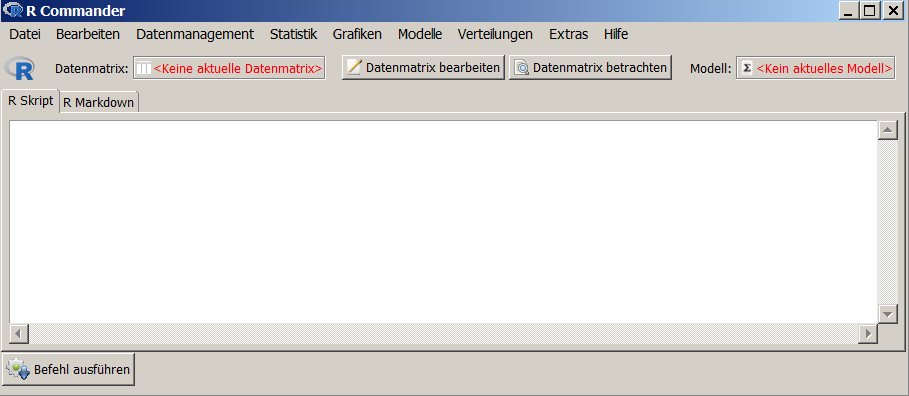
\includegraphics{figure/Rcommanderex.PNG}

\end{frame}

\begin{frame}{\href{https://gallery.shinyapps.io/cran-gauge/}{Die
Popularität von R}}
\protect\hypertarget{die-popularitat-von-r}{}

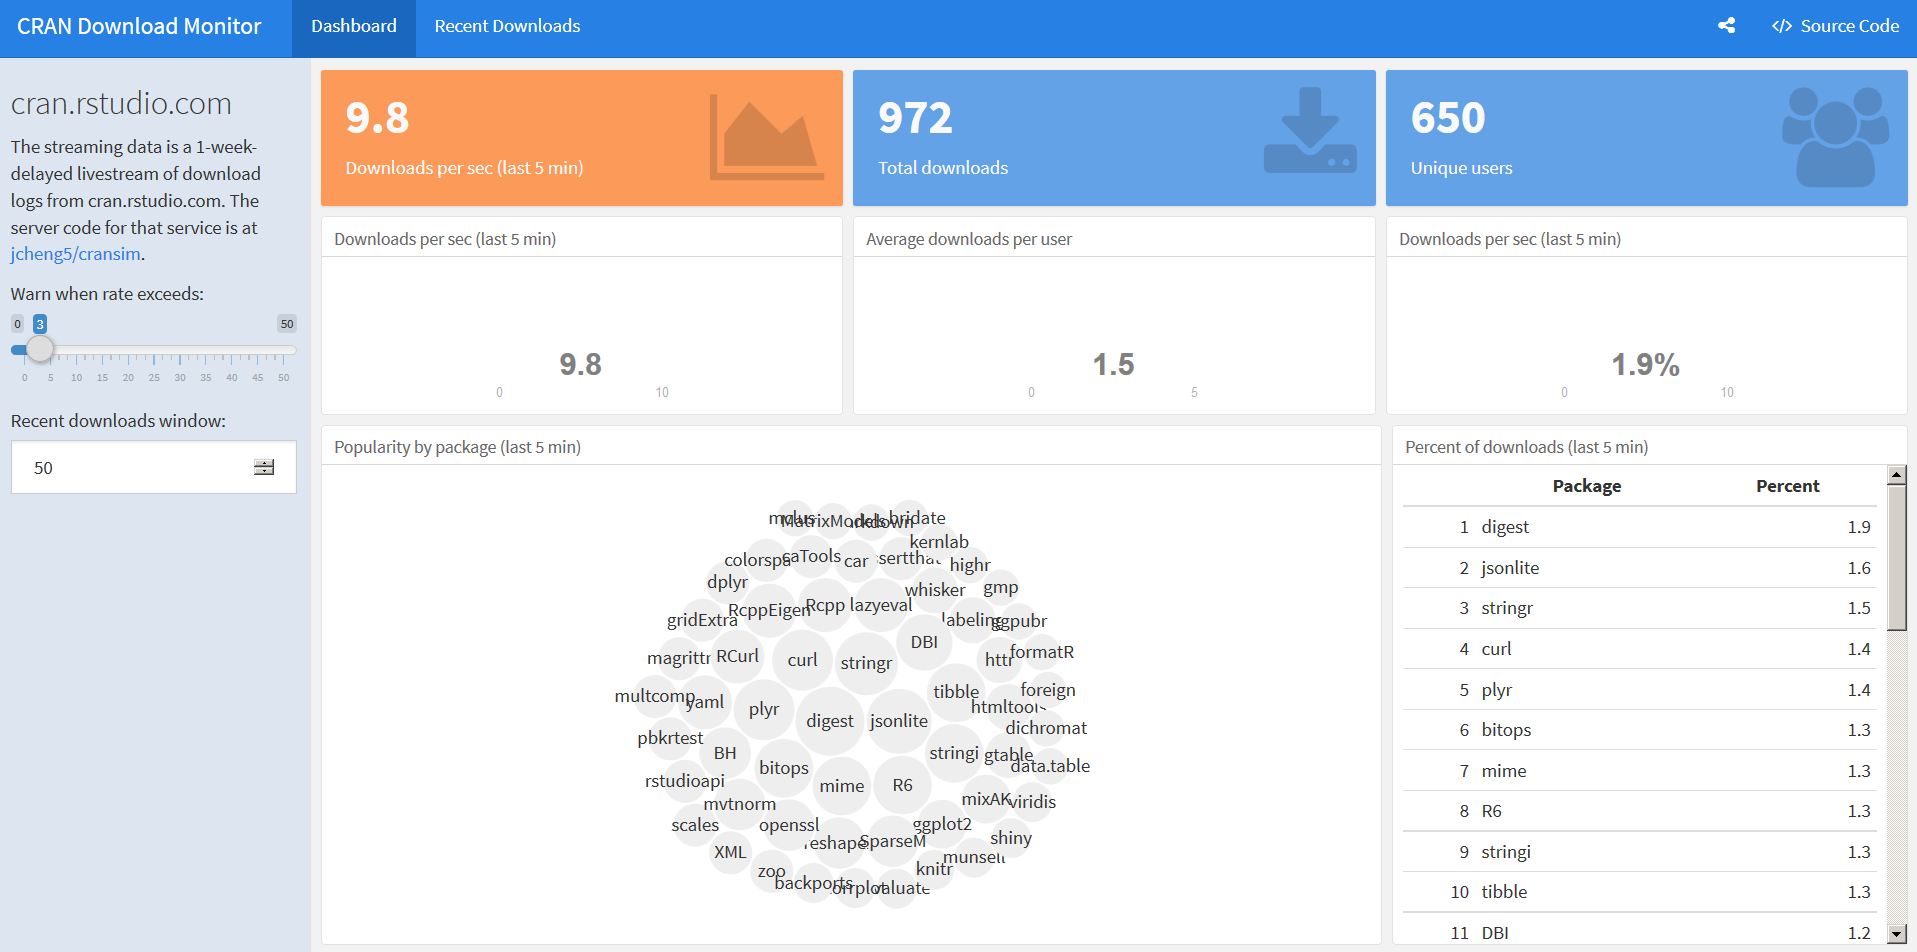
\includegraphics{figure/CRANdownloads.PNG}

\end{frame}

\begin{frame}{Erwartungen und Anforderungen}
\protect\hypertarget{erwartungen-und-anforderungen}{}

Das kann diese Schulung vermitteln:

\begin{itemize}
\tightlist
\item
  Eine praxisnahe Einführung in die statistische Programmiersprache R
\item
  Erlernen einer Programmier-Strategie
\item
  Guten Stil
\item
  Die Vorzüge graphischer Datenanalyse
\end{itemize}

\end{frame}

\begin{frame}{Erwartungen und Anforderungen II}
\protect\hypertarget{erwartungen-und-anforderungen-ii}{}

Das kann sie nicht leisten:

\begin{itemize}
\tightlist
\item
  Eine Einführungsveranstaltung in die Statistik geben
\item
  Grundlegende datenanalytische Konzepte vermitteln
\item
  Verständnis zementieren
\item
  Das Trainieren abnehmen
\end{itemize}

\end{frame}

\begin{frame}{R herunterladen:}
\protect\hypertarget{r-herunterladen}{}

\url{http://www.r-project.org/}

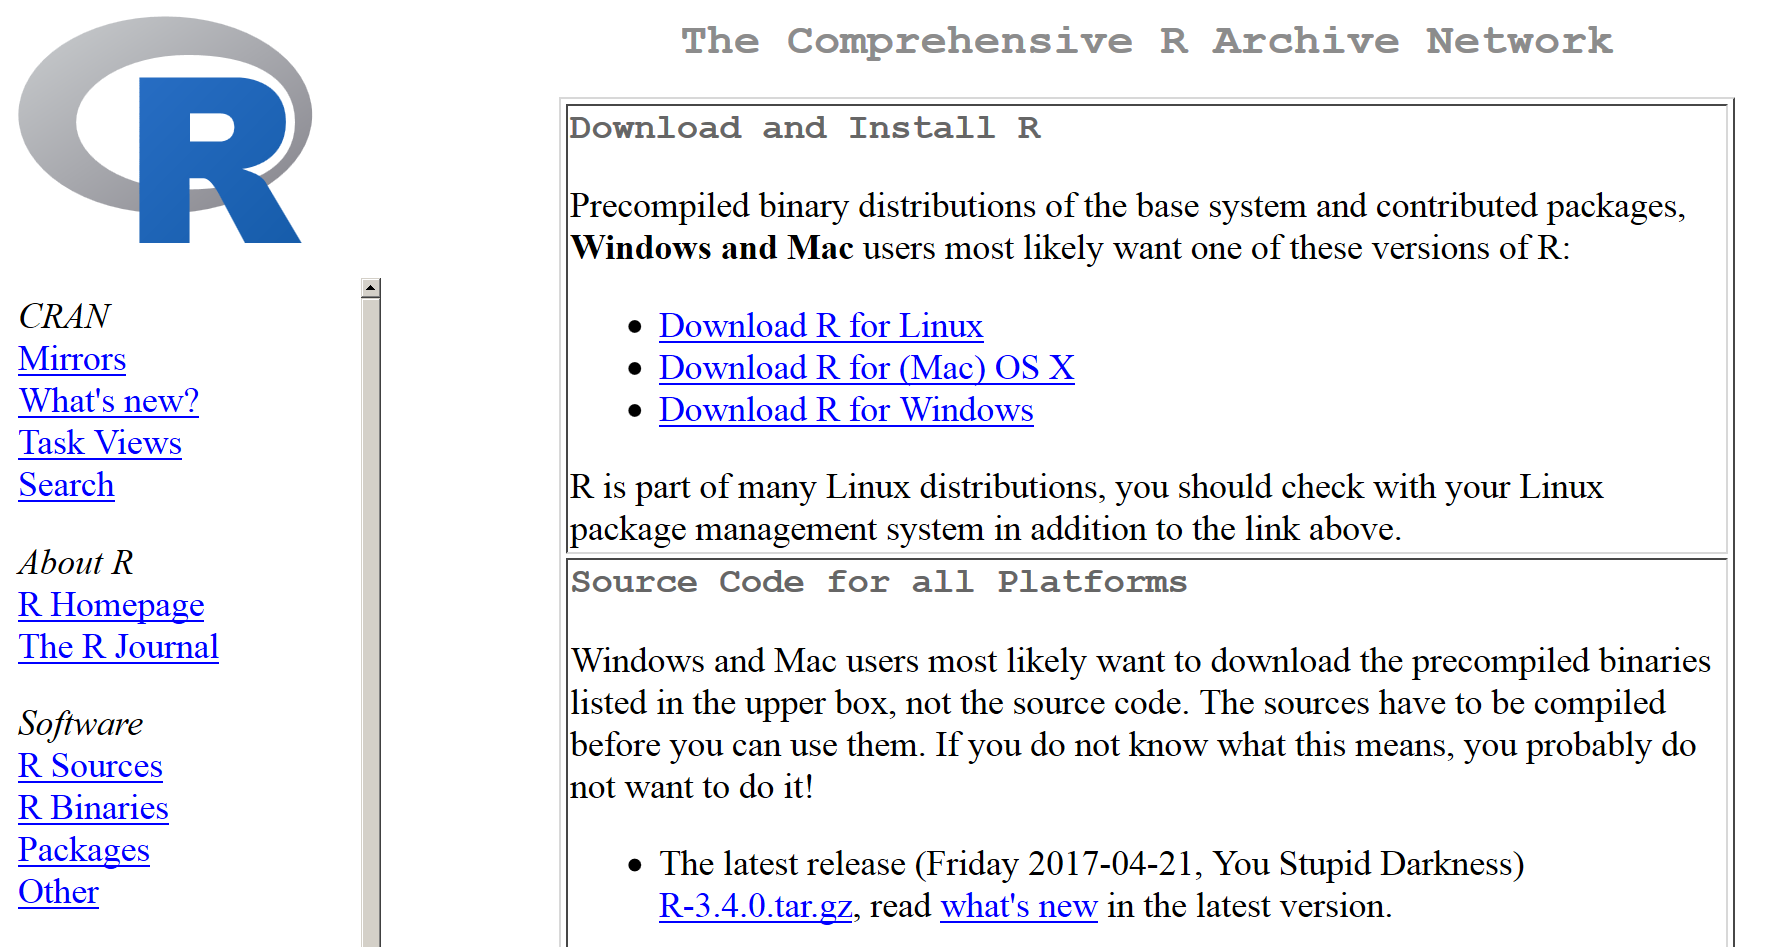
\includegraphics{figure/CRAN1picture.PNG}

\end{frame}

\begin{frame}{Links}
\protect\hypertarget{links}{}

\begin{itemize}
\item
  \href{http://www.r-bloggers.com/why-you-should-learn-r-first-for-data-science/}{Warum
  man R für Data Science lernen sollte}
\item
  \href{http://www.r-bloggers.com/rstudio-infoworld-2015-technology-of-the-year-award-recipient/}{R
  Technologie des Jahres}
\item
  \href{http://www.fastcolabs.com/3030063/why-the-r-programming-language-is-good-for-business}{Why
  R is Good for Business}
\item
  \href{http://www.r-bloggers.com/why-use-r/}{Warum R auf r-bloggers}
\item
  \href{http://www.ats.ucla.edu/stat/r/seminars/intro.htm}{Intro R}
\item
  \href{http://www.ats.ucla.edu/stat/r/sk/}{Intro R II}
\item
  \href{http://www.dataschool.io/python-or-r-for-data-science/}{Vergleich
  python und R}
\end{itemize}

\end{frame}

\begin{frame}{Probleme mit Excel}
\protect\hypertarget{probleme-mit-excel}{}

Weil andere Programme große Fehler haben:

\begin{itemize}
\item
  \href{http://blog.revolutionanalytics.com/2013/02/did-an-excel-error-bring-down-the-london-whale.html}{Excel
  bug}
\item
  \href{https://coffeehouse.dataone.org/2014/04/09/abandon-all-hope-ye-who-enter-dates-in-excel/}{Datum
  in Excel}
\end{itemize}


\includegraphics{figure/Abandon.PNG}

\end{frame}

\begin{frame}{\href{http://www.biomedcentral.com/1471-2105/5/80}{Probleme
mit Excel}}
\protect\hypertarget{probleme-mit-excel-1}{}


\includegraphics{figure/ExcelProblems.PNG}

\end{frame}

\begin{frame}{\href{https://www.inwt-statistics.de/blog-artikel-lesen/Statistik-Software-R_SAS_SPSS_STATA_im_Vergleich.html}{Vergleich
mit anderen Programmen}}
\protect\hypertarget{vergleich-mit-anderen-programmen}{}


\includegraphics{figure/SoftwareVergleich.PNG}

\end{frame}

\hypertarget{dein-freund-das-gui}{%
\section{Dein Freund das GUI}\label{dein-freund-das-gui}}

\begin{frame}{Open Source Programm R}
\protect\hypertarget{open-source-programm-r}{}

\begin{itemize}
\item
  R ist eine freie, nicht-kommerzielle Implementierung der
  Programmiersprache S (von AT\&T Bell Laboratories entwickelt)
\item
  Freie Beteiligung - modularer Aufbau (immer mehr Erweiterungspakete)
\item
  Der Download ist auf dieser Seite möglich:
\end{itemize}

\url{https://cran.r-project.org/}

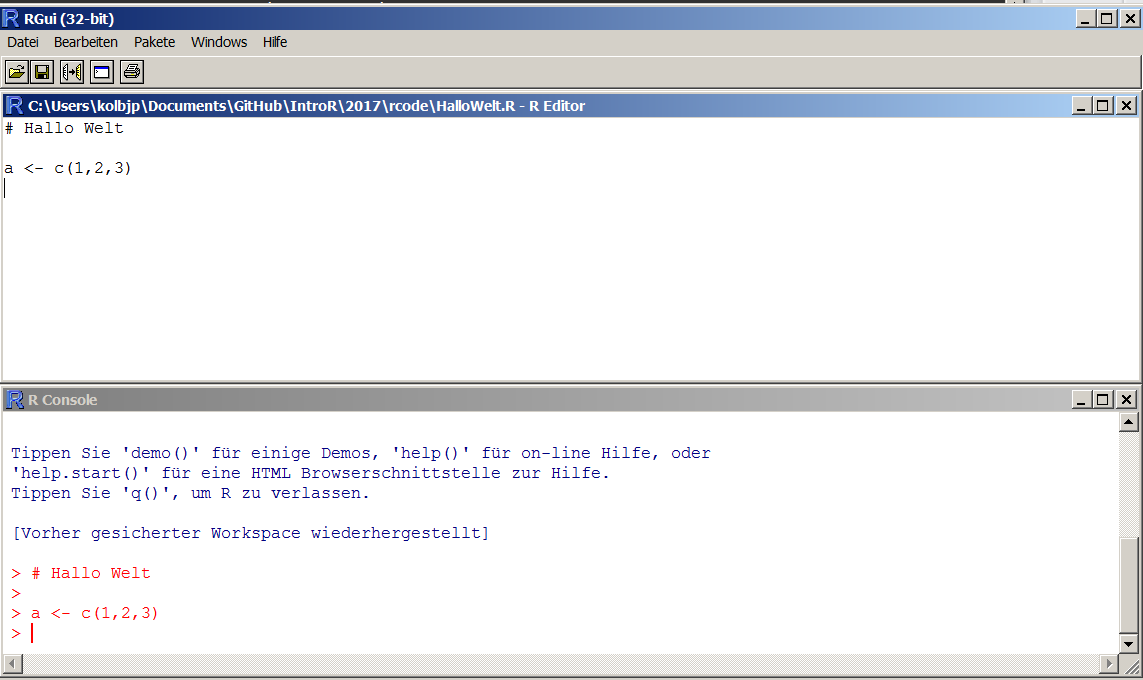
\includegraphics{figure/BasisR.PNG}

\end{frame}

\begin{frame}{Graphisches User Interface}
\protect\hypertarget{graphisches-user-interface}{}

Aber die meisten Menschen nutzen einen Editor oder ein graphical user
interface (GUI).

Aus den folgenden Gründen:

\begin{itemize}
\tightlist
\item
  Syntax highlighting
\item
  Auto-Vervollständigung
\item
  Bessere Übersicht über Graphiken, Bibliotheken
\end{itemize}

\end{frame}

\begin{frame}{Verschiedene GUIs}
\protect\hypertarget{verschiedene-guis}{}

\begin{itemize}
\item
  \href{https://projects.gnome.org/gedit/}{Gedit} mit R-spezifischen
  Add-ons für Linux
\item
  \href{http://www.gnu.org/software/emacs/}{Emacs}
\item
  \href{http://www.sciviews.org/Tinn-R/}{TinnR}
\item
  Ich nutze \href{https://www.rstudio.com/}{Rstudio!}
\end{itemize}

\begin{figure}
\centering
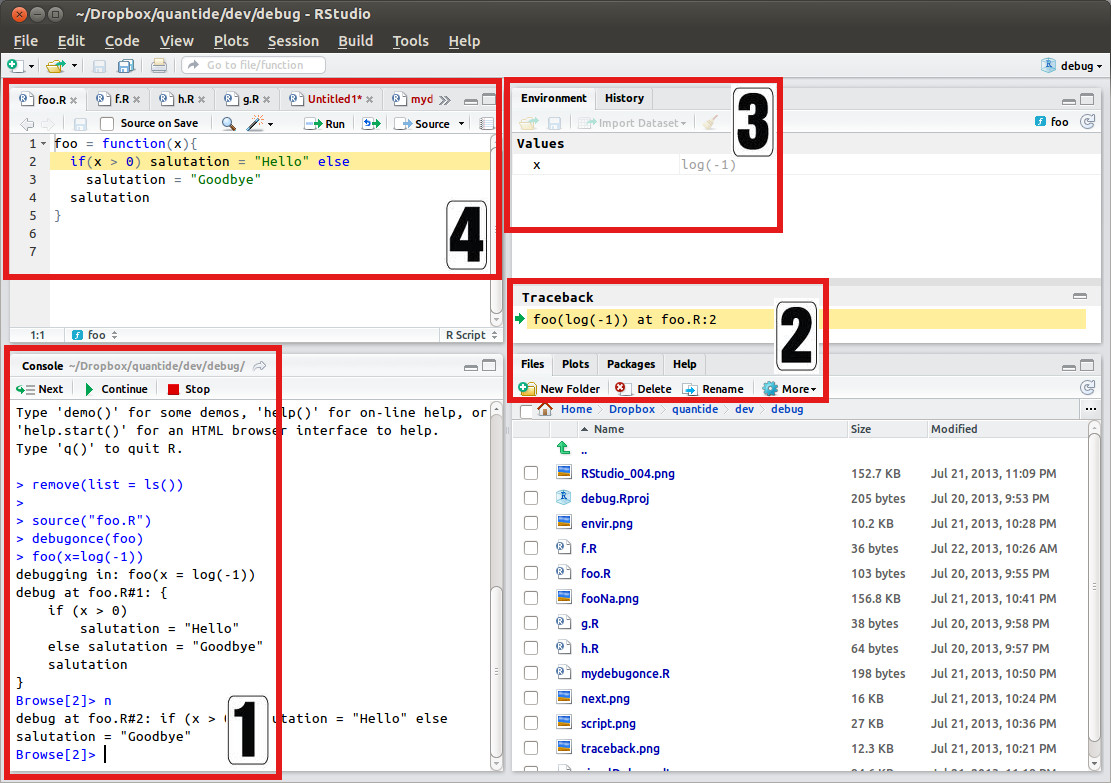
\includegraphics{figure/0_overall.jpg}
\caption{rstudio}
\end{figure}

\end{frame}

\begin{frame}{Rstudio}
\protect\hypertarget{rstudio}{}

\begin{itemize}
\item
  Sechs
  \href{http://www.r-bloggers.com/top-6-reasons-you-need-to-be-using-rstudio/}{Gründe}
  Rstudio zu nutzen.
\item
  Wie man Rstudio
  \href{https://support.rstudio.com/hc/en-us/sections/200107586-Using-RStudio}{nutzen
  kann.}
\item
  \href{https://support.rstudio.com/hc/en-us/articles/200549016-Customizing-RStudio}{Das
  Rstudio einrichten}
\end{itemize}

\end{frame}

\begin{frame}{Download der Unterlagen}
\protect\hypertarget{download-der-unterlagen}{}

Auf \href{https://github.com/Japhilko/IntroR/tree/master/2017}{github}
sind alle Unterlagen für diesen Kurs zu finden.

\href{https://guides.github.com/activities/hello-world/}{Wie nutzt man
github?}

\end{frame}

\begin{frame}[fragile]{Aufgabe - Vorbereitung}
\protect\hypertarget{aufgabe---vorbereitung}{}

\begin{itemize}
\tightlist
\item
  Prüfen Sie, ob eine Version von R auf Rechner installiert ist.
\item
  Falls dies nicht der Fall ist, laden Sie \href{r-project.org}{R}
  runter und installieren Sie R.
\item
  Prüfen Sie, ob Rstudio installiert ist.
\item
  Falls nicht - \href{http://www.rstudio.com/}{Installieren} sie
  Rstudio.
\item
  Laden Sie die R-Skripte von meinem GitHub-Account
\item
  Erstellen Sie ein erstes Script und finden Sie das Datum mit dem
  Befehl \texttt{date()} und die R-version mit \texttt{sessionInfo()}
  heraus.
\end{itemize}

\begin{Shaded}
\begin{Highlighting}[]
\KeywordTok{date}\NormalTok{()}
\end{Highlighting}
\end{Shaded}

\begin{verbatim}
## [1] "Mon May 06 10:11:04 2019"
\end{verbatim}

\begin{Shaded}
\begin{Highlighting}[]
\KeywordTok{sessionInfo}\NormalTok{()}
\end{Highlighting}
\end{Shaded}

\begin{verbatim}
## R version 3.5.0 (2018-04-23)
## Platform: x86_64-w64-mingw32/x64 (64-bit)
## Running under: Windows 7 x64 (build 7601) Service Pack 1
## 
## Matrix products: default
## 
## locale:
## [1] LC_COLLATE=German_Germany.1252  LC_CTYPE=German_Germany.1252   
## [3] LC_MONETARY=German_Germany.1252 LC_NUMERIC=C                   
## [5] LC_TIME=German_Germany.1252    
## 
## attached base packages:
## [1] stats     graphics  grDevices utils     datasets  methods   base     
## 
## loaded via a namespace (and not attached):
##  [1] compiler_3.5.0  backports_1.1.2 magrittr_1.5    rprojroot_1.3-2
##  [5] tools_3.5.0     htmltools_0.3.6 yaml_2.1.19     Rcpp_0.12.17   
##  [9] stringi_1.1.7   rmarkdown_1.10  knitr_1.20      stringr_1.4.0  
## [13] digest_0.6.18   evaluate_0.10.1
\end{verbatim}

\end{frame}

\hypertarget{grundlagen-im-umgang-mit-der-sprache-r}{%
\section{Grundlagen im Umgang mit der Sprache
R}\label{grundlagen-im-umgang-mit-der-sprache-r}}

\begin{frame}[fragile]{R ist eine Objekt-orientierte Sprache}
\protect\hypertarget{r-ist-eine-objekt-orientierte-sprache}{}

Vektoren und Zuweisungen

\begin{itemize}
\tightlist
\item
  R ist eine Objekt-orientierte Sprache
\item
  \texttt{\textless{}-} ist der Zuweisungsoperator
\end{itemize}

\begin{Shaded}
\begin{Highlighting}[]
\NormalTok{b <-}\StringTok{ }\KeywordTok{c}\NormalTok{(}\DecValTok{1}\NormalTok{,}\DecValTok{2}\NormalTok{) }\CommentTok{# erzeugt ein Objekt mit den Zahlen 1 und 2}
\end{Highlighting}
\end{Shaded}

\begin{itemize}
\tightlist
\item
  Eine Funktion kann auf dieses Objekt angewendet werden:
\end{itemize}

\begin{Shaded}
\begin{Highlighting}[]
\KeywordTok{mean}\NormalTok{(b) }\CommentTok{# berechnet den Mittelwert}
\end{Highlighting}
\end{Shaded}

\begin{verbatim}
## [1] 1.5
\end{verbatim}

Mit den folgenden Funktionen können wir etwas über die Eigenschaften des
Objekts lernen:

\begin{Shaded}
\begin{Highlighting}[]
\KeywordTok{length}\NormalTok{(b) }\CommentTok{# b hat die Länge 2}
\end{Highlighting}
\end{Shaded}

\begin{verbatim}
## [1] 2
\end{verbatim}

\end{frame}

\begin{frame}[fragile]{Objektstruktur}
\protect\hypertarget{objektstruktur}{}

\begin{Shaded}
\begin{Highlighting}[]
\KeywordTok{str}\NormalTok{(b) }\CommentTok{# b ist ein numerischer Vektor}
\end{Highlighting}
\end{Shaded}

\begin{verbatim}
##  num [1:2] 1 2
\end{verbatim}

\end{frame}

\begin{frame}{Funktionen im base-Paket}
\protect\hypertarget{funktionen-im-base-paket}{}

\begin{longtable}[]{@{}lll@{}}
\toprule
Funktion & Bedeutung & Beispiel\tabularnewline
\midrule
\endhead
length() & Länge & length(b)\tabularnewline
max() & Maximum & max(b)\tabularnewline
min() & Minimum & min(b)\tabularnewline
sd() & Standardabweichung & sd(b)\tabularnewline
var() & Varianz & var(b)\tabularnewline
mean() & Mittelwert & mean(b)\tabularnewline
median() & Median & median(b)\tabularnewline
\bottomrule
\end{longtable}

Diese Funktionen brauchen nur ein Argument.

\end{frame}

\begin{frame}{Funktionen mit mehr Argumenten}
\protect\hypertarget{funktionen-mit-mehr-argumenten}{}

Andere Funktionen brauchen mehr:

\begin{longtable}[]{@{}lll@{}}
\toprule
Argument & Bedeutung & Beispiel\tabularnewline
\midrule
\endhead
quantile() & 90 \% Quantile & quantile(b,.9)\tabularnewline
sample() & Stichprobe ziehen & sample(b,1)\tabularnewline
\bottomrule
\end{longtable}

\end{frame}

\begin{frame}[fragile]{Beispiel - Funktionen mit einem Argument}
\protect\hypertarget{beispiel---funktionen-mit-einem-argument}{}

\begin{Shaded}
\begin{Highlighting}[]
\KeywordTok{max}\NormalTok{(b)}
\end{Highlighting}
\end{Shaded}

\begin{verbatim}
## [1] 2
\end{verbatim}

\begin{Shaded}
\begin{Highlighting}[]
\KeywordTok{min}\NormalTok{(b)}
\end{Highlighting}
\end{Shaded}

\begin{verbatim}
## [1] 1
\end{verbatim}

\begin{Shaded}
\begin{Highlighting}[]
\KeywordTok{sd}\NormalTok{(b)}
\end{Highlighting}
\end{Shaded}

\begin{verbatim}
## [1] 0.7071068
\end{verbatim}

\begin{Shaded}
\begin{Highlighting}[]
\KeywordTok{var}\NormalTok{(b)}
\end{Highlighting}
\end{Shaded}

\begin{verbatim}
## [1] 0.5
\end{verbatim}

\end{frame}

\begin{frame}[fragile]{Funktionen mit einem Argument}
\protect\hypertarget{funktionen-mit-einem-argument}{}

\begin{Shaded}
\begin{Highlighting}[]
\KeywordTok{mean}\NormalTok{(b)}
\end{Highlighting}
\end{Shaded}

\begin{verbatim}
## [1] 1.5
\end{verbatim}

\begin{Shaded}
\begin{Highlighting}[]
\KeywordTok{median}\NormalTok{(b)}
\end{Highlighting}
\end{Shaded}

\begin{verbatim}
## [1] 1.5
\end{verbatim}

\end{frame}

\begin{frame}[fragile]{Funktionen mit mehr Argumenten}
\protect\hypertarget{funktionen-mit-mehr-argumenten-1}{}

\begin{Shaded}
\begin{Highlighting}[]
\KeywordTok{quantile}\NormalTok{(b,.}\DecValTok{9}\NormalTok{)}
\end{Highlighting}
\end{Shaded}

\begin{verbatim}
## 90% 
## 1.9
\end{verbatim}

\begin{Shaded}
\begin{Highlighting}[]
\KeywordTok{sample}\NormalTok{(b,}\DecValTok{1}\NormalTok{) }
\end{Highlighting}
\end{Shaded}

\begin{verbatim}
## [1] 1
\end{verbatim}

\end{frame}

\begin{frame}{\href{http://cran.r-project.org/doc/manuals/R-intro.html}{Übersicht
Befehle}}
\protect\hypertarget{ubersicht-befehle}{}

\url{http://cran.r-project.org/doc/manuals/R-intro.html}

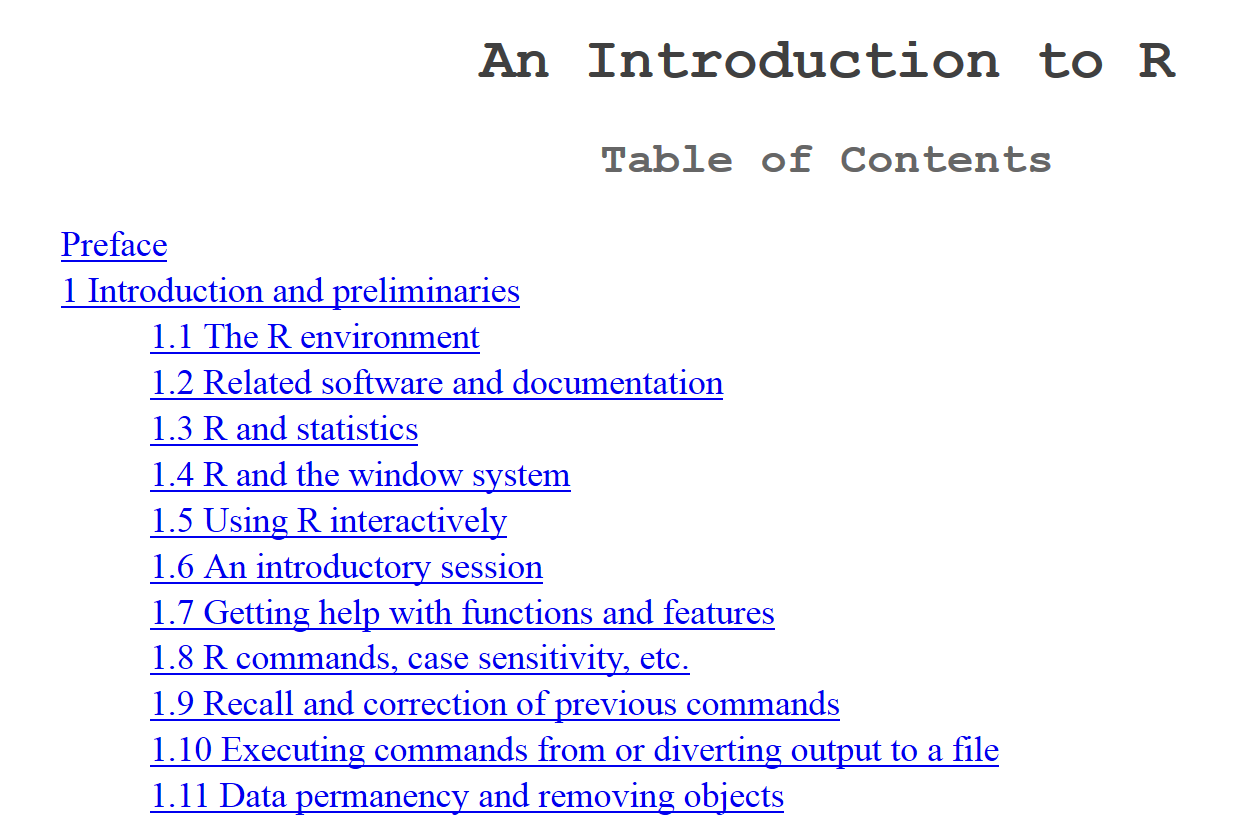
\includegraphics{figure/UebersichtBefehle.PNG}

\end{frame}

\begin{frame}{Aufgabe - Zuweisungen und Funktionen}
\protect\hypertarget{aufgabe---zuweisungen-und-funktionen}{}

Erzeugen Sie einen Vektor b mit den Zahlen von 1 bis 5 und berechnen
Sie\ldots{}

\begin{enumerate}
\item
  den Mittelwert
\item
  die Varianz
\item
  die Standardabweichung
\item
  die quadratische Wurzel aus dem Mittelwert
\end{enumerate}

\end{frame}

\hypertarget{datentypen-und-indizieren}{%
\section{Datentypen und Indizieren}\label{datentypen-und-indizieren}}

\begin{frame}[fragile]{Verschiedene Datentypen}
\protect\hypertarget{verschiedene-datentypen}{}

\begin{longtable}[]{@{}lll@{}}
\toprule
Datentyp & Beschreibung & Beispiel\tabularnewline
\midrule
\endhead
numeric & ganze und reele Zahlen & \texttt{5,\ 3.462}\tabularnewline
logical & logische Werte & \texttt{FALSE,\ TRUE}\tabularnewline
character & Buchstaben und Zeichenfolgen &
\texttt{"Hallo"}\tabularnewline
\bottomrule
\end{longtable}

Quelle:
\href{https://www.uni-trier.de/fileadmin/fb4/prof/VWL/FIN/Oekonometrie/PC-UEbung/Einfuehrung_in_R.pdf}{R.
Münnich und M. Knobelspieß} (2007): Einführung in das statistische
Programmpaket R

\end{frame}

\begin{frame}[fragile]{Verschiedene Datentypen}
\protect\hypertarget{verschiedene-datentypen-1}{}

\begin{Shaded}
\begin{Highlighting}[]
\NormalTok{b <-}\StringTok{ }\KeywordTok{c}\NormalTok{(}\DecValTok{1}\NormalTok{,}\DecValTok{2}\NormalTok{) }\CommentTok{# numeric}
\NormalTok{log <-}\StringTok{ }\KeywordTok{c}\NormalTok{(T,F) }\CommentTok{# logical}
\NormalTok{char <-}\KeywordTok{c}\NormalTok{(}\StringTok{"A"}\NormalTok{,}\StringTok{"b"}\NormalTok{) }\CommentTok{# character}
\NormalTok{fac <-}\StringTok{ }\KeywordTok{as.factor}\NormalTok{(}\KeywordTok{c}\NormalTok{(}\DecValTok{1}\NormalTok{,}\DecValTok{2}\NormalTok{)) }\CommentTok{# factor}
\end{Highlighting}
\end{Shaded}

Mit \texttt{str()} bekommt man den Objekttyp.

\begin{Shaded}
\begin{Highlighting}[]
\KeywordTok{str}\NormalTok{(fac)}
\end{Highlighting}
\end{Shaded}

\begin{verbatim}
##  Factor w/ 2 levels "1","2": 1 2
\end{verbatim}

\end{frame}

\begin{frame}[fragile]{Indizieren eines Vektors:}
\protect\hypertarget{indizieren-eines-vektors}{}

\begin{Shaded}
\begin{Highlighting}[]
\NormalTok{A1 <-}\StringTok{ }\KeywordTok{c}\NormalTok{(}\DecValTok{1}\NormalTok{,}\DecValTok{2}\NormalTok{,}\DecValTok{3}\NormalTok{,}\DecValTok{4}\NormalTok{)}
\NormalTok{A1}
\end{Highlighting}
\end{Shaded}

\begin{verbatim}
## [1] 1 2 3 4
\end{verbatim}

\begin{Shaded}
\begin{Highlighting}[]
\NormalTok{A1[}\DecValTok{1}\NormalTok{]}
\end{Highlighting}
\end{Shaded}

\begin{verbatim}
## [1] 1
\end{verbatim}

\begin{Shaded}
\begin{Highlighting}[]
\NormalTok{A1[}\DecValTok{4}\NormalTok{]}
\end{Highlighting}
\end{Shaded}

\begin{verbatim}
## [1] 4
\end{verbatim}

\begin{Shaded}
\begin{Highlighting}[]
\NormalTok{A1[}\DecValTok{1}\OperatorTok{:}\DecValTok{3}\NormalTok{]}
\end{Highlighting}
\end{Shaded}

\begin{verbatim}
## [1] 1 2 3
\end{verbatim}

\begin{Shaded}
\begin{Highlighting}[]
\NormalTok{A1[}\OperatorTok{-}\DecValTok{4}\NormalTok{]}
\end{Highlighting}
\end{Shaded}

\begin{verbatim}
## [1] 1 2 3
\end{verbatim}

\end{frame}

\begin{frame}[fragile]{data.frames}
\protect\hypertarget{data.frames}{}

Beispieldaten generieren:

\begin{Shaded}
\begin{Highlighting}[]
\NormalTok{AGE <-}\StringTok{ }\KeywordTok{c}\NormalTok{(}\DecValTok{20}\NormalTok{,}\DecValTok{35}\NormalTok{,}\DecValTok{48}\NormalTok{,}\DecValTok{12}\NormalTok{)}
\NormalTok{SEX <-}\StringTok{ }\KeywordTok{c}\NormalTok{(}\StringTok{"m"}\NormalTok{,}\StringTok{"w"}\NormalTok{,}\StringTok{"w"}\NormalTok{,}\StringTok{"m"}\NormalTok{)}
\end{Highlighting}
\end{Shaded}

Diese beiden Vektoren zu einem data.frame verbinden:

\begin{Shaded}
\begin{Highlighting}[]
\NormalTok{Daten <-}\StringTok{ }\KeywordTok{data.frame}\NormalTok{(}\DataTypeTok{Alter=}\NormalTok{AGE,}\DataTypeTok{Geschlecht=}\NormalTok{SEX)}
\end{Highlighting}
\end{Shaded}

Anzahl der Zeilen/Spalten herausfinden

\begin{Shaded}
\begin{Highlighting}[]
\KeywordTok{nrow}\NormalTok{(Daten) }\CommentTok{# Zeilen}
\end{Highlighting}
\end{Shaded}

\begin{verbatim}
## [1] 4
\end{verbatim}

\begin{Shaded}
\begin{Highlighting}[]
\KeywordTok{ncol}\NormalTok{(Daten) }\CommentTok{# Spalten}
\end{Highlighting}
\end{Shaded}

\begin{verbatim}
## [1] 2
\end{verbatim}

\end{frame}

\begin{frame}[fragile]{Indizieren}
\protect\hypertarget{indizieren}{}

Indizieren eines dataframe:

\begin{Shaded}
\begin{Highlighting}[]
\NormalTok{AA <-}\StringTok{ }\DecValTok{4}\OperatorTok{:}\DecValTok{1}
\NormalTok{A2 <-}\StringTok{ }\KeywordTok{cbind}\NormalTok{(A1,AA)}
\NormalTok{A2[}\DecValTok{1}\NormalTok{,}\DecValTok{1}\NormalTok{]}
\end{Highlighting}
\end{Shaded}

\begin{verbatim}
## A1 
##  1
\end{verbatim}

\begin{Shaded}
\begin{Highlighting}[]
\NormalTok{A2[}\DecValTok{2}\NormalTok{,]}
\end{Highlighting}
\end{Shaded}

\begin{verbatim}
## A1 AA 
##  2  3
\end{verbatim}

\begin{Shaded}
\begin{Highlighting}[]
\NormalTok{A2[,}\DecValTok{1}\NormalTok{]}
\end{Highlighting}
\end{Shaded}

\begin{verbatim}
## [1] 1 2 3 4
\end{verbatim}

\begin{Shaded}
\begin{Highlighting}[]
\NormalTok{A2[,}\DecValTok{1}\OperatorTok{:}\DecValTok{2}\NormalTok{]}
\end{Highlighting}
\end{Shaded}

\begin{verbatim}
##      A1 AA
## [1,]  1  4
## [2,]  2  3
## [3,]  3  2
## [4,]  4  1
\end{verbatim}

\end{frame}

\begin{frame}[fragile]{Matrizen und Arrays}
\protect\hypertarget{matrizen-und-arrays}{}

\begin{itemize}
\tightlist
\item
  In Matrizen und Arrays stehen meist nur numerische Werte.
\item
  Dadurch wird beispielsweise Matrix Multiplikation möglich.
\item
  Anders als beim data.frame sind mehr als zwei Dimensionen möglich.
\end{itemize}

\begin{Shaded}
\begin{Highlighting}[]
\NormalTok{A <-}\StringTok{ }\KeywordTok{matrix}\NormalTok{(}\KeywordTok{seq}\NormalTok{(}\DecValTok{1}\NormalTok{,}\DecValTok{100}\NormalTok{), }\DataTypeTok{nrow =} \DecValTok{4}\NormalTok{)}
\KeywordTok{dim}\NormalTok{(A)}
\end{Highlighting}
\end{Shaded}

\begin{verbatim}
## [1]  4 25
\end{verbatim}

\end{frame}

\begin{frame}[fragile]{Ein Array erzeugen}
\protect\hypertarget{ein-array-erzeugen}{}

\begin{Shaded}
\begin{Highlighting}[]
\NormalTok{A3 <-}\StringTok{ }\KeywordTok{array}\NormalTok{(}\DecValTok{1}\OperatorTok{:}\DecValTok{8}\NormalTok{,}\KeywordTok{c}\NormalTok{(}\DecValTok{2}\NormalTok{,}\DecValTok{2}\NormalTok{,}\DecValTok{2}\NormalTok{))}
\NormalTok{A3}
\end{Highlighting}
\end{Shaded}

\begin{verbatim}
## , , 1
## 
##      [,1] [,2]
## [1,]    1    3
## [2,]    2    4
## 
## , , 2
## 
##      [,1] [,2]
## [1,]    5    7
## [2,]    6    8
\end{verbatim}

\end{frame}

\begin{frame}[fragile]{Indizieren eines Array}
\protect\hypertarget{indizieren-eines-array}{}

\begin{Shaded}
\begin{Highlighting}[]
\NormalTok{A3[,,}\DecValTok{2}\NormalTok{]}
\end{Highlighting}
\end{Shaded}

\begin{verbatim}
##      [,1] [,2]
## [1,]    5    7
## [2,]    6    8
\end{verbatim}

\end{frame}

\begin{frame}{Listen}
\protect\hypertarget{listen}{}

\begin{itemize}
\tightlist
\item
  Eine Liste in R entspricht einem geschachtelten Array in anderen
  Programmiersprachen
\item
  Listen können alles enthalten
\item
  Listen können geschachtelt sein
\item
  Listen sollte man sehr bedacht verwenden
\end{itemize}

\end{frame}

\begin{frame}[fragile]{Indizieren einer Liste}
\protect\hypertarget{indizieren-einer-liste}{}

\begin{Shaded}
\begin{Highlighting}[]
\NormalTok{A4 <-}\StringTok{ }\KeywordTok{list}\NormalTok{(A1,}\DecValTok{1}\NormalTok{)}
\NormalTok{A4}
\end{Highlighting}
\end{Shaded}

\begin{verbatim}
## [[1]]
## [1] 1 2 3 4
## 
## [[2]]
## [1] 1
\end{verbatim}

\begin{Shaded}
\begin{Highlighting}[]
\NormalTok{A4[[}\DecValTok{2}\NormalTok{]]}
\end{Highlighting}
\end{Shaded}

\begin{verbatim}
## [1] 1
\end{verbatim}

\end{frame}

\begin{frame}[fragile]{Logische Operatoren}
\protect\hypertarget{logische-operatoren}{}

\begin{Shaded}
\begin{Highlighting}[]
\CommentTok{# Ist 1 größer als 2?}
\DecValTok{1}\OperatorTok{>}\DecValTok{2}
\end{Highlighting}
\end{Shaded}

\begin{verbatim}
## [1] FALSE
\end{verbatim}

\begin{Shaded}
\begin{Highlighting}[]
\DecValTok{1}\OperatorTok{<}\DecValTok{2}
\end{Highlighting}
\end{Shaded}

\begin{verbatim}
## [1] TRUE
\end{verbatim}

\begin{Shaded}
\begin{Highlighting}[]
\DecValTok{1}\OperatorTok{==}\DecValTok{2}
\end{Highlighting}
\end{Shaded}

\begin{verbatim}
## [1] FALSE
\end{verbatim}

\end{frame}

\begin{frame}[fragile]{Operatoren um Subset für Datensatz zu bekommen}
\protect\hypertarget{operatoren-um-subset-fur-datensatz-zu-bekommen}{}

Diese Operatoren eignen sich gut um Datensätze einzuschränken

\begin{Shaded}
\begin{Highlighting}[]
\NormalTok{Daten}
\end{Highlighting}
\end{Shaded}

\begin{verbatim}
##   Alter Geschlecht
## 1    20          m
## 2    35          w
## 3    48          w
## 4    12          m
\end{verbatim}

\begin{Shaded}
\begin{Highlighting}[]
\NormalTok{Daten[AGE}\OperatorTok{>}\DecValTok{20}\NormalTok{,]}
\end{Highlighting}
\end{Shaded}

\begin{verbatim}
##   Alter Geschlecht
## 2    35          w
## 3    48          w
\end{verbatim}

\end{frame}

\begin{frame}[fragile]{Datensätze einschränken}
\protect\hypertarget{datensatze-einschranken}{}

\begin{Shaded}
\begin{Highlighting}[]
\NormalTok{Daten[SEX}\OperatorTok{==}\StringTok{"w"}\NormalTok{,]}
\end{Highlighting}
\end{Shaded}

\begin{verbatim}
##   Alter Geschlecht
## 2    35          w
## 3    48          w
\end{verbatim}

\begin{Shaded}
\begin{Highlighting}[]
\CommentTok{# gleiches Ergebnis:}
\NormalTok{Daten[SEX}\OperatorTok{!=}\StringTok{"m"}\NormalTok{,]}
\end{Highlighting}
\end{Shaded}

\begin{verbatim}
##   Alter Geschlecht
## 2    35          w
## 3    48          w
\end{verbatim}

\end{frame}

\begin{frame}[fragile]{Weitere wichtige Optionen}
\protect\hypertarget{weitere-wichtige-optionen}{}

\begin{Shaded}
\begin{Highlighting}[]
\CommentTok{# Ergebnis in ein Objekt speichern}
\NormalTok{subDat <-}\StringTok{ }\NormalTok{Daten[AGE}\OperatorTok{>}\DecValTok{20}\NormalTok{,]}
\end{Highlighting}
\end{Shaded}

\begin{Shaded}
\begin{Highlighting}[]
\CommentTok{# mehrere Bedingeungen können mit}
\CommentTok{# & verknüpft werden:}
\NormalTok{Daten[AGE}\OperatorTok{>}\DecValTok{18} \OperatorTok{&}\StringTok{ }\NormalTok{SEX}\OperatorTok{==}\StringTok{"w"}\NormalTok{,]}
\end{Highlighting}
\end{Shaded}

\begin{verbatim}
##   Alter Geschlecht
## 2    35          w
## 3    48          w
\end{verbatim}

\end{frame}

\begin{frame}[fragile]{Sequenzen}
\protect\hypertarget{sequenzen}{}

\begin{Shaded}
\begin{Highlighting}[]
\CommentTok{# Sequenz von 1 bis 10}
\DecValTok{1}\OperatorTok{:}\DecValTok{10}
\end{Highlighting}
\end{Shaded}

\begin{verbatim}
##  [1]  1  2  3  4  5  6  7  8  9 10
\end{verbatim}

\begin{Shaded}
\begin{Highlighting}[]
\NormalTok{Daten[}\DecValTok{1}\OperatorTok{:}\DecValTok{3}\NormalTok{,]}
\end{Highlighting}
\end{Shaded}

\begin{verbatim}
##   Alter Geschlecht
## 1    20          m
## 2    35          w
## 3    48          w
\end{verbatim}

\end{frame}

\begin{frame}[fragile]{Weitere Sequenzen}
\protect\hypertarget{weitere-sequenzen}{}

\begin{Shaded}
\begin{Highlighting}[]
\KeywordTok{seq}\NormalTok{(}\OperatorTok{-}\DecValTok{2}\NormalTok{,}\DecValTok{8}\NormalTok{,}\DataTypeTok{by=}\FloatTok{1.5}\NormalTok{)}
\end{Highlighting}
\end{Shaded}

\begin{verbatim}
## [1] -2.0 -0.5  1.0  2.5  4.0  5.5  7.0
\end{verbatim}

\begin{Shaded}
\begin{Highlighting}[]
\NormalTok{a <-}\KeywordTok{seq}\NormalTok{(}\DecValTok{3}\NormalTok{,}\DecValTok{12}\NormalTok{,}\DataTypeTok{length=}\DecValTok{12}\NormalTok{)}

\NormalTok{b <-}\StringTok{ }\KeywordTok{seq}\NormalTok{(}\DataTypeTok{to=}\DecValTok{5}\NormalTok{,}\DataTypeTok{length=}\DecValTok{12}\NormalTok{,}\DataTypeTok{by=}\FloatTok{0.2}\NormalTok{)}

\NormalTok{d <-}\StringTok{ }\DecValTok{1}\OperatorTok{:}\DecValTok{10}
\NormalTok{d <-}\StringTok{ }\KeywordTok{seq}\NormalTok{(}\DecValTok{1}\NormalTok{,}\DecValTok{10}\NormalTok{,}\DecValTok{1}\NormalTok{)}
\NormalTok{d <-}\StringTok{ }\KeywordTok{seq}\NormalTok{(}\DataTypeTok{length=}\DecValTok{10}\NormalTok{,}\DataTypeTok{from=}\DecValTok{1}\NormalTok{,}\DataTypeTok{by=}\DecValTok{1}\NormalTok{)}
\end{Highlighting}
\end{Shaded}

\end{frame}

\begin{frame}[fragile]{Wiederholungen}
\protect\hypertarget{wiederholungen}{}

\begin{Shaded}
\begin{Highlighting}[]
\CommentTok{# wiederhole 1 10 mal}
\KeywordTok{rep}\NormalTok{(}\DecValTok{1}\NormalTok{,}\DecValTok{10}\NormalTok{)}
\end{Highlighting}
\end{Shaded}

\begin{verbatim}
##  [1] 1 1 1 1 1 1 1 1 1 1
\end{verbatim}

\begin{Shaded}
\begin{Highlighting}[]
\KeywordTok{rep}\NormalTok{(}\StringTok{"A"}\NormalTok{,}\DecValTok{10}\NormalTok{)}
\end{Highlighting}
\end{Shaded}

\begin{verbatim}
##  [1] "A" "A" "A" "A" "A" "A" "A" "A" "A" "A"
\end{verbatim}

\end{frame}

\begin{frame}[fragile]{Die Funktion paste}
\protect\hypertarget{die-funktion-paste}{}

\begin{Shaded}
\begin{Highlighting}[]
\NormalTok{?paste}
\end{Highlighting}
\end{Shaded}

\begin{Shaded}
\begin{Highlighting}[]
\KeywordTok{paste}\NormalTok{(}\DecValTok{1}\OperatorTok{:}\DecValTok{4}\NormalTok{)}
\end{Highlighting}
\end{Shaded}

\begin{verbatim}
## [1] "1" "2" "3" "4"
\end{verbatim}

\begin{Shaded}
\begin{Highlighting}[]
\KeywordTok{paste}\NormalTok{(}\StringTok{"A"}\NormalTok{, }\DecValTok{1}\OperatorTok{:}\DecValTok{6}\NormalTok{, }\DataTypeTok{sep =} \StringTok{""}\NormalTok{)}
\end{Highlighting}
\end{Shaded}

\begin{verbatim}
## [1] "A1" "A2" "A3" "A4" "A5" "A6"
\end{verbatim}

\begin{itemize}
\tightlist
\item
  Ein weiteres Beispiel:
\end{itemize}

\begin{Shaded}
\begin{Highlighting}[]
\KeywordTok{paste0}\NormalTok{(}\StringTok{"A"}\NormalTok{, }\DecValTok{1}\OperatorTok{:}\DecValTok{6}\NormalTok{)}
\end{Highlighting}
\end{Shaded}

\begin{verbatim}
## [1] "A1" "A2" "A3" "A4" "A5" "A6"
\end{verbatim}

\end{frame}

\hypertarget{wie-bekommt-man-hilfe}{%
\section{Wie bekommt man Hilfe?}\label{wie-bekommt-man-hilfe}}

\begin{frame}[fragile]{Wie bekommt man Hilfe?}
\protect\hypertarget{wie-bekommt-man-hilfe-1}{}

\begin{itemize}
\tightlist
\item
  \href{http://itfeature.com/tag/how-to-get-help-in-r}{Um generell Hilfe
  zu bekommen:}
\end{itemize}

\begin{Shaded}
\begin{Highlighting}[]
\KeywordTok{help.start}\NormalTok{()}
\end{Highlighting}
\end{Shaded}

\begin{itemize}
\tightlist
\item
  Online Dokumentation für die meisten Funktionen:
\end{itemize}

\begin{Shaded}
\begin{Highlighting}[]
\KeywordTok{help}\NormalTok{(name)}
\end{Highlighting}
\end{Shaded}

\begin{itemize}
\tightlist
\item
  Nutze ? um Hilfe zu bekommen.
\end{itemize}

\begin{Shaded}
\begin{Highlighting}[]
\NormalTok{?mean}
\end{Highlighting}
\end{Shaded}

\begin{itemize}
\tightlist
\item
  example(lm) gibt ein Beispiel für die lineare Regression
\end{itemize}

\begin{Shaded}
\begin{Highlighting}[]
\KeywordTok{example}\NormalTok{(lm)}
\end{Highlighting}
\end{Shaded}

\end{frame}

\begin{frame}[fragile]{Nutzung Suchmaschinen}
\protect\hypertarget{nutzung-suchmaschinen}{}

\begin{itemize}
\tightlist
\item
  Ich nutze meistens google
\item
  Tippe:
\end{itemize}

\begin{verbatim}
R-project + Was ich schon immer wissen wollte
\end{verbatim}

\begin{itemize}
\tightlist
\item
  Das funktioniert natürlich mit jeder Suchmaschine!
\end{itemize}

\end{frame}

\begin{frame}{\href{http://stackoverflow.com/}{Stackoverflow}}
\protect\hypertarget{stackoverflow}{}

\begin{itemize}
\tightlist
\item
  Für Fragen zum Programmieren
\item
  Ist nicht auf R fokussiert
\item
  Sehr detailierte Diskussionen
\end{itemize}

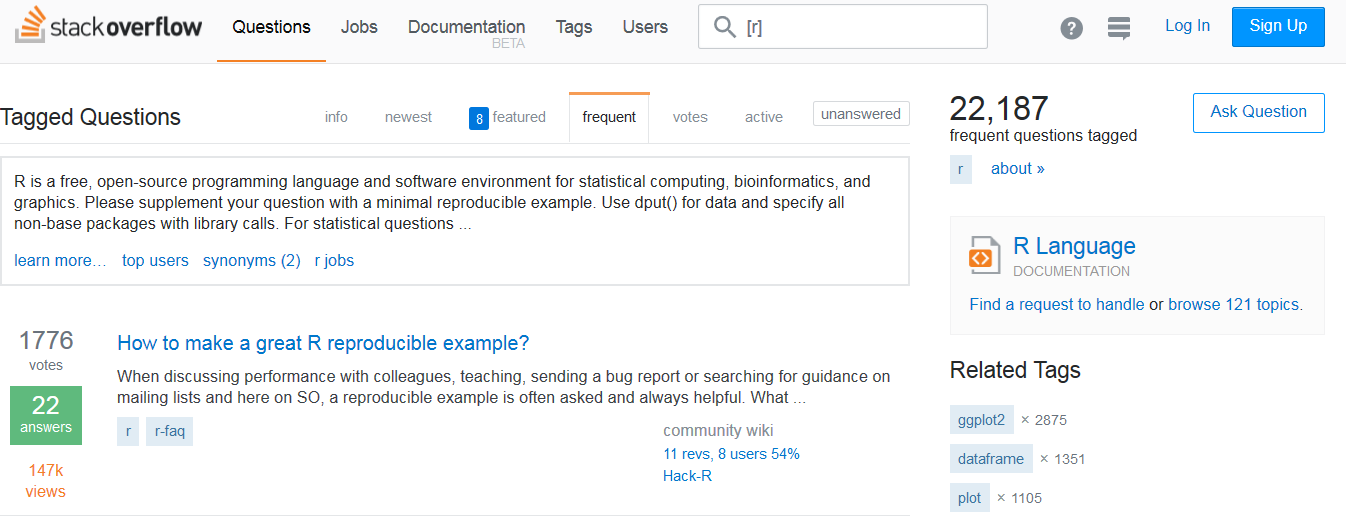
\includegraphics{https://github.com/Japhilko/IntroR/blob/master/2017/slides/figure/StackoverflowEx.PNG?raw=true}

\end{frame}

\begin{frame}{Ein Schummelzettel - Cheatsheet}
\protect\hypertarget{ein-schummelzettel---cheatsheet}{}

\url{https://www.rstudio.com/resources/cheatsheets/}

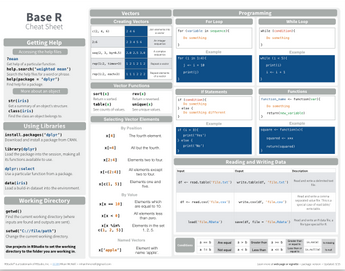
\includegraphics{https://github.com/Japhilko/IntroR/blob/master/2017/slides/figure/cheatsheetBaseR.PNG?raw=true}

\end{frame}

\hypertarget{modularer-aufbau-von-r}{%
\section{Modularer Aufbau von R}\label{modularer-aufbau-von-r}}

\begin{frame}{Modularer Aufbau}
\protect\hypertarget{modularer-aufbau}{}

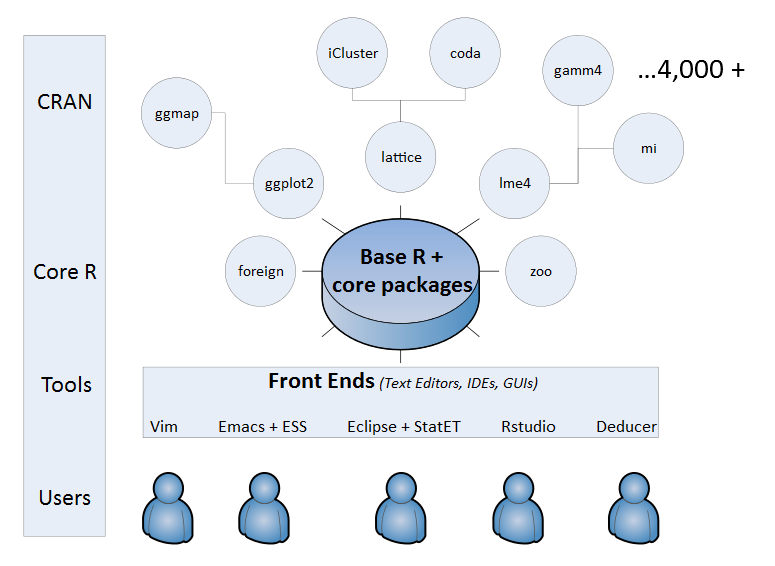
\includegraphics{figure/Packages.PNG}

\end{frame}

\begin{frame}[fragile]{Modularer Aufbau}
\protect\hypertarget{modularer-aufbau-1}{}

\begin{itemize}
\tightlist
\item
  Viele Funktionen sind im Basis-R enthalten
\item
  Viele spezifische Funktionen sind in zusätzlichen Bibliotheken
  integriert
\item
  R kann modular erweitert werden durch sog. packages bzw. libraries
\item
  Auf CRAN werden die wichtigsten packages gehostet (im Moment 10430)
\item
  Weitergehende Pakete finden sich z.B. bei
  \href{www.bioconductor.org}{bioconductor}
\end{itemize}

\begin{Shaded}
\begin{Highlighting}[]
\KeywordTok{install.packages}\NormalTok{(}\StringTok{"lme4"}\NormalTok{)}

\KeywordTok{library}\NormalTok{(lme4)}
\end{Highlighting}
\end{Shaded}

\end{frame}

\begin{frame}{Installation von Paketen mit RStudio}
\protect\hypertarget{installation-von-paketen-mit-rstudio}{}

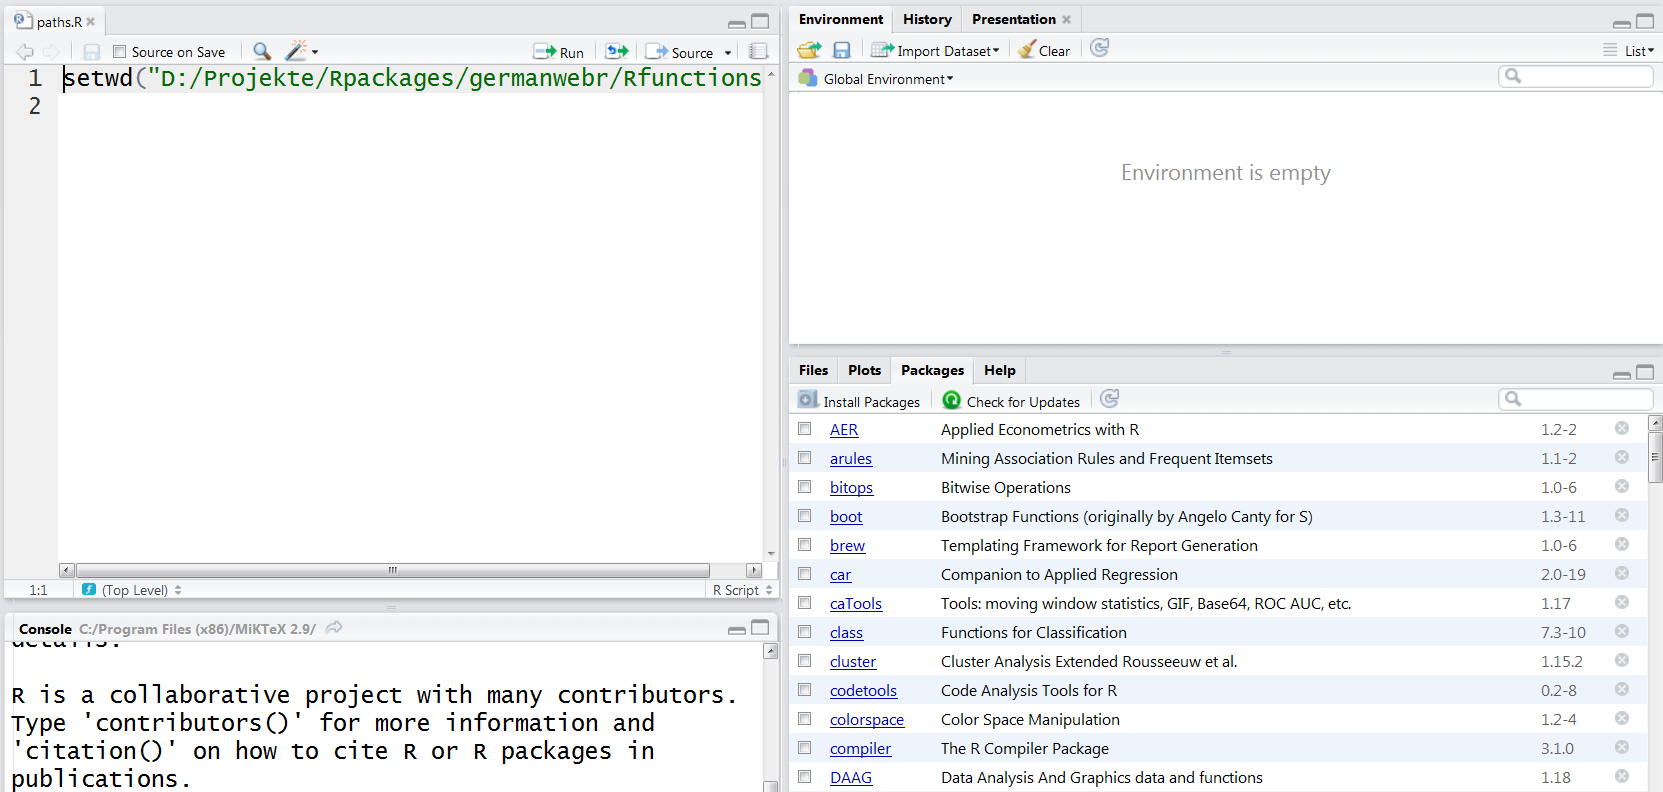
\includegraphics{figure/PaketeRstudio.PNG}

\end{frame}

\begin{frame}{Vorhandene Pakete und Installation}
\protect\hypertarget{vorhandene-pakete-und-installation}{}

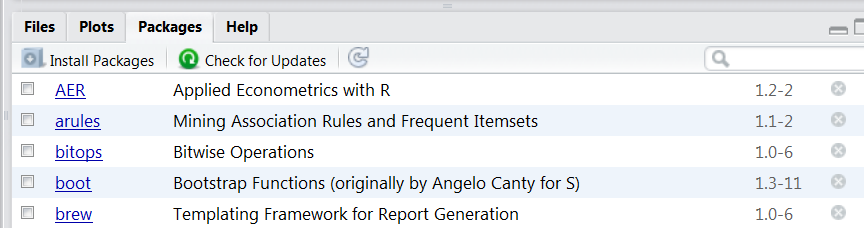
\includegraphics{figure/packages3.PNG}

\end{frame}

\begin{frame}[fragile]{Übersicht viele nützliche Pakete:}
\protect\hypertarget{ubersicht-viele-nutzliche-pakete}{}

\begin{itemize}
\tightlist
\item
  Luhmann -
  \href{http://www.beltz.de/fileadmin/beltz/downloads/OnlinematerialienPVU/28090_Luhmann/Verwendete\%20Pakete.pdf}{Tabelle
  mit vielen nützlichen Paketen}
\end{itemize}

Weitere interessante Pakete:

\begin{itemize}
\item
  Paket für den Import/Export -
  \href{http://cran.r-project.org/web/packages/foreign/foreign.pdf}{foreign}
\item
  \href{http://iase-web.org/documents/papers/icots8/ICOTS8_4J1_TILLE.pdf}{Pakete
  für Survey Sampling}
\item
  \texttt{xtable} Paket für die Integration von Latex und R
  (\href{http://cran.r-project.org/web/packages/xtable/vignettes/xtableGallery.pdf}{xtable
  Galerie})
\item
  \href{http://cran.r-project.org/web/packages/dummies/dummies.pdf}{Paket
  zur Erzeugung von Dummies}
\item
  \href{http://cran.r-project.org/web/packages/mvtnorm/index.html}{Multivariate
  Normalverteilung}
\item
  \href{http://www.r-bloggers.com/tag/maptools/}{Paket für Karten}
\end{itemize}

\end{frame}

\begin{frame}[fragile]{Pakete von Github installieren}
\protect\hypertarget{pakete-von-github-installieren}{}

\begin{Shaded}
\begin{Highlighting}[]
\KeywordTok{install.packages}\NormalTok{(}\StringTok{"devtools"}\NormalTok{)}
\KeywordTok{library}\NormalTok{(devtools)}

\KeywordTok{install_github}\NormalTok{(}\StringTok{"hadley/ggplot2"}\NormalTok{)}
\end{Highlighting}
\end{Shaded}

\end{frame}

\begin{frame}{Wie bekomme ich einen Überblick}
\protect\hypertarget{wie-bekomme-ich-einen-uberblick}{}

\begin{itemize}
\item
  \href{https://mran.microsoft.com/packages/}{Explore Packages Currently
  on CRAN}
\item
  \href{https://gallery.shinyapps.io/cran-gauge/}{Pakete die in letzter
  Zeit von CRAN heruntergeladen wurden}
\end{itemize}

\end{frame}

\begin{frame}{Aufgabe - Zusatzpakete}
\protect\hypertarget{aufgabe---zusatzpakete}{}

Gehen Sie auf \url{https://cran.r-project.org/} und suchen Sie in dem
Bereich, wo die Pakete vorgestellt werden, nach Paketen,\ldots{}

\begin{itemize}
\tightlist
\item
  die für die deskriptive Datenanalyse geeignet sind.
\item
  um Regressionen zu berechnen
\item
  um fremde Datensätze einzulesen (z.B. SPSS-Daten)
\item
  um mit großen Datenmengen umzugehen
\end{itemize}

\end{frame}

\hypertarget{datenimport}{%
\section{Datenimport}\label{datenimport}}

\begin{frame}{Datenimport}
\protect\hypertarget{datenimport-1}{}

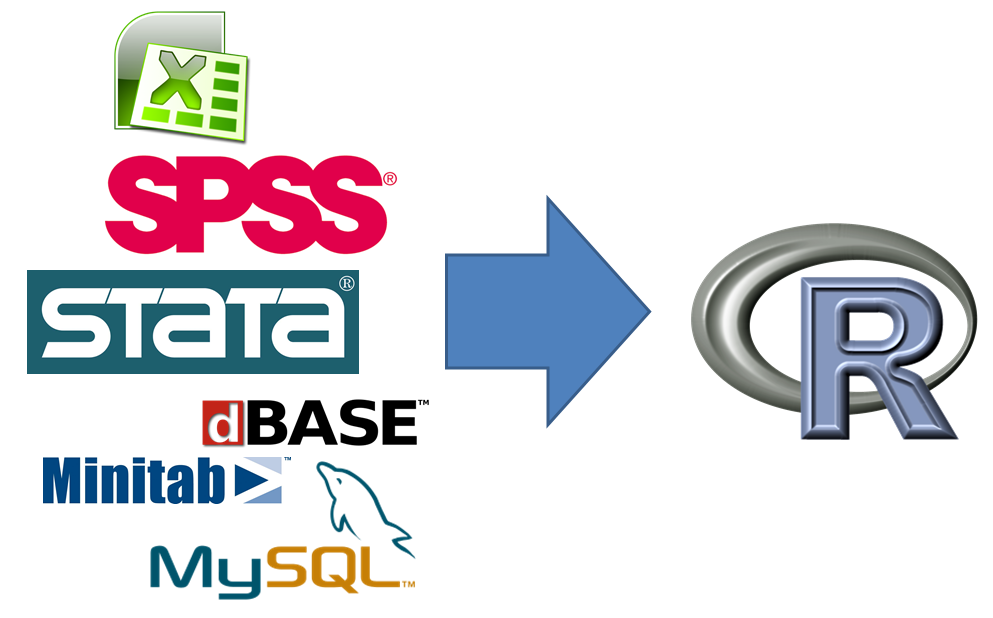
\includegraphics{figure/Datenimport.PNG}

\end{frame}

\begin{frame}{Dateiformate in R}
\protect\hypertarget{dateiformate-in-r}{}

\begin{itemize}
\tightlist
\item
  Von R werden quelloffene, nicht-proprietäre Formate bevorzugt
\item
  Es können aber auch Formate von anderen Statistik Software Paketen
  eingelesen werden
\item
  R-user speichern Objekte gerne in sog. Workspaces ab
\item
  Auch hier jedoch gilt: (fast) alles andere ist möglich
\end{itemize}

\end{frame}

\begin{frame}[fragile]{Formate - base package}
\protect\hypertarget{formate---base-package}{}

R unterstützt von Haus aus schon einige wichtige Formate:

\begin{itemize}
\tightlist
\item
  CSV (Comma Separated Values): \texttt{read.csv()}
\item
  FWF (Fixed With Format): \texttt{read.fwf()}
\item
  Tab-getrennte Werte: \texttt{read.delim()}
\end{itemize}

\end{frame}

\begin{frame}[fragile]{Der Arbeitsspeicher}
\protect\hypertarget{der-arbeitsspeicher}{}

So findet man heraus, in welchem Verzeichnis man sich gerade befindet

\begin{Shaded}
\begin{Highlighting}[]
\KeywordTok{getwd}\NormalTok{()}
\end{Highlighting}
\end{Shaded}

So kann man das Arbeitsverzeichnis ändern:

Man erzeugt ein Objekt in dem man den Pfad abspeichert:

\begin{Shaded}
\begin{Highlighting}[]
\NormalTok{main.path <-}\StringTok{ "C:/"} \CommentTok{# Beispiel für Windows}
\NormalTok{main.path <-}\StringTok{ "/users/Name/"} \CommentTok{# Beispiel für Mac}
\NormalTok{main.path <-}\StringTok{ "/home/user/"} \CommentTok{# Beispiel für Linux}
\end{Highlighting}
\end{Shaded}

Und ändert dann den Pfad mit setwd()

\begin{Shaded}
\begin{Highlighting}[]
\KeywordTok{setwd}\NormalTok{(main.path)}
\end{Highlighting}
\end{Shaded}

Bei Windows ist es wichtig Slashs anstelle von Backslashs zu verwenden.

\end{frame}

\begin{frame}{Alternative - Arbeitsspeicher}
\protect\hypertarget{alternative---arbeitsspeicher}{}

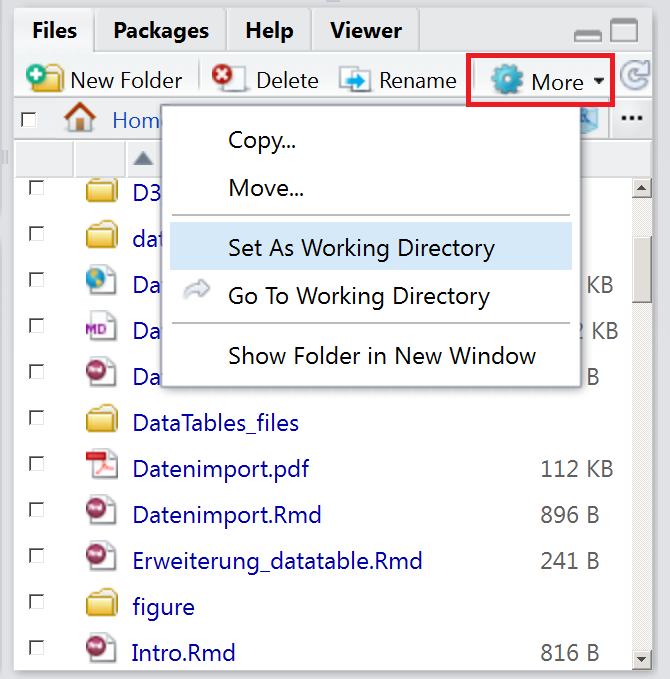
\includegraphics{figure/SetWD.PNG}

\end{frame}

\begin{frame}[fragile]{Import von Excel-Daten}
\protect\hypertarget{import-von-excel-daten}{}

\begin{itemize}
\tightlist
\item
  \texttt{library(foreign)} ist für den Import von fremden Datenformaten
  nötig
\item
  Wenn Excel-Daten vorliegen - als .csv abspeichern
\item
  Dann kann \texttt{read.csv()} genutzt werden um die Daten einzulesen.
\item
  Bei Deutschen Daten kann es sein, dass man \texttt{read.csv2()} wegen
  der Komma-Separierung braucht.
\end{itemize}

\begin{Shaded}
\begin{Highlighting}[]
\KeywordTok{library}\NormalTok{(foreign)}
\NormalTok{?read.csv}
\NormalTok{?read.csv2}
\end{Highlighting}
\end{Shaded}

\end{frame}

\begin{frame}[fragile]{CSV Dateien einlesen}
\protect\hypertarget{csv-dateien-einlesen}{}

Zunächst muss das Arbeitsverzeichnis gesetzt werden, in dem sich die
Daten befinden:

\begin{Shaded}
\begin{Highlighting}[]
\NormalTok{Dat <-}\StringTok{ }\KeywordTok{read.csv}\NormalTok{(}\StringTok{"schuldaten_export.csv"}\NormalTok{)}
\end{Highlighting}
\end{Shaded}

Wenn es sich um Deutsche Daten handelt:

\begin{Shaded}
\begin{Highlighting}[]
\NormalTok{Dat <-}\StringTok{ }\KeywordTok{read.csv2}\NormalTok{(}\StringTok{"schuldaten_export.csv"}\NormalTok{)}
\end{Highlighting}
\end{Shaded}

\end{frame}

\begin{frame}[fragile]{SPSS Dateien einlesen}
\protect\hypertarget{spss-dateien-einlesen}{}

Dateien können auch direkt aus dem Internet geladen werden:

\begin{Shaded}
\begin{Highlighting}[]
\NormalTok{link<-}\StringTok{ "http://www.statistik.at/web_de/static/}
\StringTok{mz_2013_sds_-_datensatz_080469.sav"}

\NormalTok{?read.spss}
\NormalTok{Dat <-}\StringTok{ }\KeywordTok{read.spss}\NormalTok{(link,}\DataTypeTok{to.data.frame=}\NormalTok{T)}
\end{Highlighting}
\end{Shaded}

\end{frame}

\begin{frame}[fragile]{stata Dateien einlesen}
\protect\hypertarget{stata-dateien-einlesen}{}

\begin{Shaded}
\begin{Highlighting}[]
\NormalTok{MZ02 <-}\StringTok{ }\KeywordTok{read.dta}\NormalTok{(}\StringTok{"MZ02.dta"}\NormalTok{)}
\end{Highlighting}
\end{Shaded}

\begin{itemize}
\tightlist
\item
  Einführung in Import mit R
  (\href{http://is-r.tumblr.com/post/37181850668/reading-writing-stata-dta-files-with-foreign}{is.R})
\end{itemize}

\end{frame}

\begin{frame}[fragile]{\href{https://cran.r-project.org/web/packages/rio/vignettes/rio.html}{Das
Paket \texttt{rio}}}
\protect\hypertarget{das-paket-rio}{}

\begin{Shaded}
\begin{Highlighting}[]
\KeywordTok{install.packages}\NormalTok{(}\StringTok{"rio"}\NormalTok{)}
\end{Highlighting}
\end{Shaded}

\begin{Shaded}
\begin{Highlighting}[]
\KeywordTok{library}\NormalTok{(}\StringTok{"rio"}\NormalTok{)}
\NormalTok{x <-}\StringTok{ }\KeywordTok{import}\NormalTok{(}\StringTok{"mtcars.csv"}\NormalTok{)}
\NormalTok{y <-}\StringTok{ }\KeywordTok{import}\NormalTok{(}\StringTok{"mtcars.rds"}\NormalTok{)}
\NormalTok{z <-}\StringTok{ }\KeywordTok{import}\NormalTok{(}\StringTok{"mtcars.dta"}\NormalTok{)}
\end{Highlighting}
\end{Shaded}

\begin{itemize}
\tightlist
\item
  \href{https://cran.r-project.org/web/packages/rio/README.html}{rio: A
  Swiss-Army Knife for Data I/O}
\end{itemize}

\end{frame}

\begin{frame}[fragile]{Datenmanagement ähnlich wie in SPSS oder Stata}
\protect\hypertarget{datenmanagement-ahnlich-wie-in-spss-oder-stata}{}

\begin{Shaded}
\begin{Highlighting}[]
\KeywordTok{install.packages}\NormalTok{(}\StringTok{"Rz"}\NormalTok{)}
\KeywordTok{library}\NormalTok{(Rz)}
\end{Highlighting}
\end{Shaded}

\end{frame}

\begin{frame}[fragile]{\href{https://cran.r-project.org/web/packages/Rcmdr/index.html}{Weitere
Alternative Rcmdr}}
\protect\hypertarget{weitere-alternative-rcmdr}{}

\begin{Shaded}
\begin{Highlighting}[]
\KeywordTok{install.packages}\NormalTok{(}\StringTok{"Rcmdr"}\NormalTok{)}
\end{Highlighting}
\end{Shaded}

\begin{itemize}
\tightlist
\item
  \href{http://www.rcommander.com/}{Funktioniert auch mit Rstudio}
\end{itemize}

\begin{Shaded}
\begin{Highlighting}[]
\KeywordTok{library}\NormalTok{(Rcmdr)}
\end{Highlighting}
\end{Shaded}

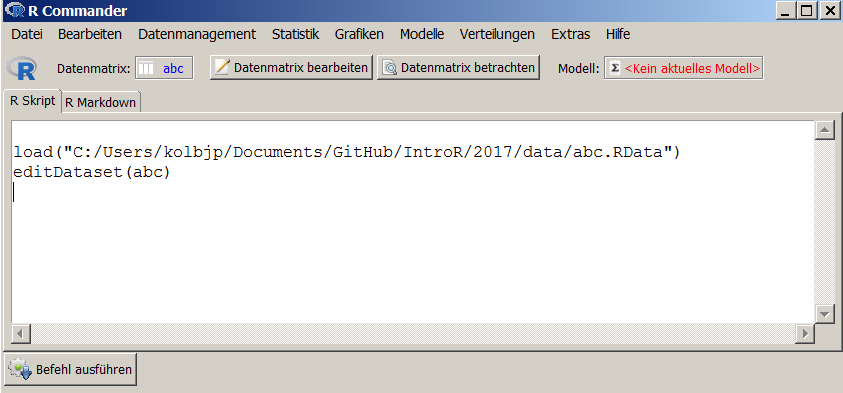
\includegraphics{figure/Rcommander.PNG}

\end{frame}

\begin{frame}{Aufgabe - Datenimport}
\protect\hypertarget{aufgabe---datenimport}{}

\begin{itemize}
\item
  Gehen Sie auf
  \href{https://github.com/Japhilko/IntroR/blob/master/2017/data/oecd.dta?raw=true}{meine
  Github Seite} und laden Sie den OECD Datensatz herunter
\item
  Laden Sie den Datensatz mit einer geeigneten Funktion in Ihre Console.
\item
  Finden Sie heraus, wieviele Beobachtungen und Variablen der Datensatz
  umfasst.
\end{itemize}

\end{frame}

\hypertarget{datenexport}{%
\section{Datenexport}\label{datenexport}}

\begin{frame}{Datenexport}
\protect\hypertarget{datenexport-1}{}

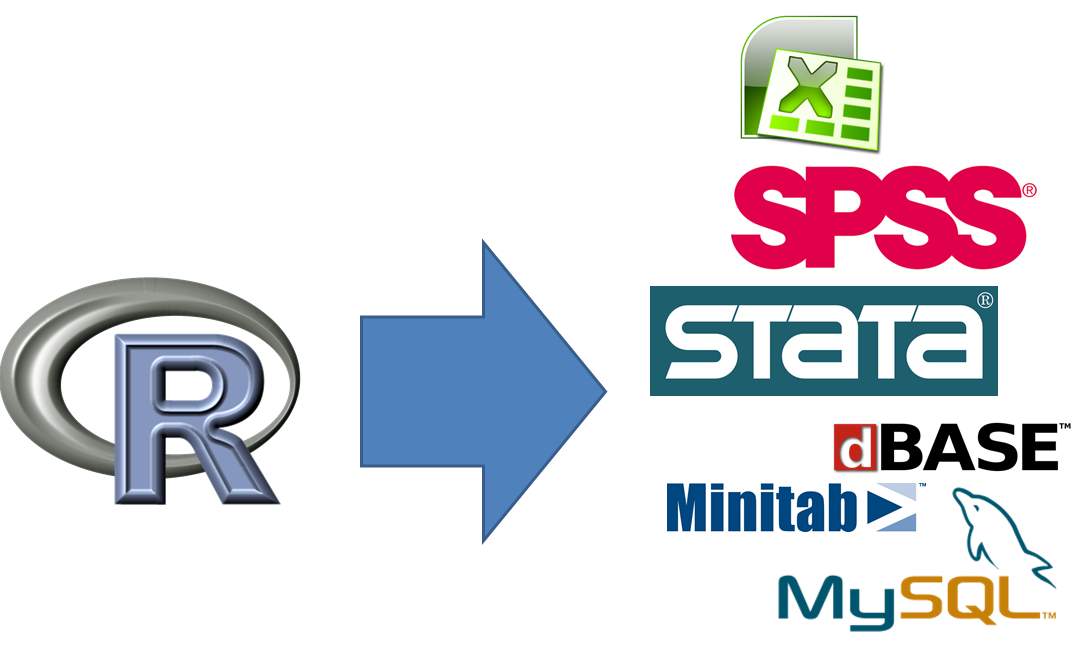
\includegraphics{figure/Datenexport.PNG}

\end{frame}

\begin{frame}[fragile]{R's Exportformate}
\protect\hypertarget{rs-exportformate}{}

\begin{itemize}
\tightlist
\item
  In R werden offene Dateiformate bevorzugt
\item
  Als Äquivalenz zu den \texttt{read.X()} Funktionen stehen viele
  \texttt{write.X()} Funktionen zur Verfügung
\item
  Das eigene Format von R sind sog. Workspaces (\texttt{.RData})
\end{itemize}

\end{frame}

\begin{frame}[fragile]{Beispieldatensatz erzeugen}
\protect\hypertarget{beispieldatensatz-erzeugen}{}

\begin{Shaded}
\begin{Highlighting}[]
\NormalTok{A <-}\StringTok{ }\KeywordTok{c}\NormalTok{(}\DecValTok{1}\NormalTok{,}\DecValTok{2}\NormalTok{,}\DecValTok{3}\NormalTok{,}\DecValTok{4}\NormalTok{)}
\NormalTok{B <-}\StringTok{ }\KeywordTok{c}\NormalTok{(}\StringTok{"A"}\NormalTok{,}\StringTok{"B"}\NormalTok{,}\StringTok{"C"}\NormalTok{,}\StringTok{"D"}\NormalTok{)}

\NormalTok{mydata <-}\StringTok{ }\KeywordTok{data.frame}\NormalTok{(A,B)}
\end{Highlighting}
\end{Shaded}

\end{frame}

\begin{frame}[fragile]{Überblick Daten Import/Export}
\protect\hypertarget{uberblick-daten-importexport}{}

\begin{Shaded}
\begin{Highlighting}[]
\KeywordTok{save}\NormalTok{(mydata, }\DataTypeTok{file=}\StringTok{"mydata.RData"}\NormalTok{)}
\end{Highlighting}
\end{Shaded}

\end{frame}

\begin{frame}[fragile]{Daten in Excel Format abspeichern}
\protect\hypertarget{daten-in-excel-format-abspeichern}{}

\begin{Shaded}
\begin{Highlighting}[]
\KeywordTok{write.csv}\NormalTok{(mydata,}\DataTypeTok{file=}\StringTok{"mydata.csv"}\NormalTok{) }
\end{Highlighting}
\end{Shaded}

\begin{Shaded}
\begin{Highlighting}[]
\KeywordTok{library}\NormalTok{(xlsx)}
\KeywordTok{write.xlsx}\NormalTok{(mydata,}\DataTypeTok{file=}\StringTok{"mydata.xlsx"}\NormalTok{) }
\end{Highlighting}
\end{Shaded}

\end{frame}

\begin{frame}[fragile]{Daten in stata Format abspeichern}
\protect\hypertarget{daten-in-stata-format-abspeichern}{}

\begin{Shaded}
\begin{Highlighting}[]
\KeywordTok{library}\NormalTok{(foreign)}
\KeywordTok{write.dta}\NormalTok{(mydata,}\DataTypeTok{file=}\StringTok{"mydata.dta"}\NormalTok{) }
\end{Highlighting}
\end{Shaded}

\end{frame}

\begin{frame}[fragile]{Auch zum Export eignet sich das \texttt{rio}
Paket}
\protect\hypertarget{auch-zum-export-eignet-sich-das-rio-paket}{}

\begin{Shaded}
\begin{Highlighting}[]
\KeywordTok{library}\NormalTok{(}\StringTok{"rio"}\NormalTok{)}

\KeywordTok{export}\NormalTok{(mtcars, }\StringTok{"mtcars.csv"}\NormalTok{)}
\KeywordTok{export}\NormalTok{(mtcars, }\StringTok{"mtcars.rds"}\NormalTok{)}
\KeywordTok{export}\NormalTok{(mtcars, }\StringTok{"mtcars.dta"}\NormalTok{)}
\end{Highlighting}
\end{Shaded}

\end{frame}

\begin{frame}{Links Export}
\protect\hypertarget{links-export}{}

\begin{itemize}
\item
  \href{http://www.statmethods.net/input/exportingdata.html}{Quick R}
  für das Exportieren von Daten:
\item
  Hilfe zum Export auf dem
  \href{http://cran.r-project.org/doc/manuals/r-release/R-data.pdf}{CRAN
  Server}
\end{itemize}

\end{frame}

\hypertarget{datenanalyse}{%
\section{Datenanalyse}\label{datenanalyse}}

\begin{frame}[fragile]{Streuungsmaße}
\protect\hypertarget{streuungsmae}{}

In Basis R sind die wichtigsten Streuungsmaße enthalten:

\begin{itemize}
\tightlist
\item
  Varianz: \texttt{var()}
\item
  Standardabweichung: \texttt{sd()}
\item
  Minimum und Maximum: \texttt{min()} und \texttt{max()}
\item
  Range: \texttt{range()}
\end{itemize}

\begin{Shaded}
\begin{Highlighting}[]
\NormalTok{ab <-}\StringTok{ }\KeywordTok{rnorm}\NormalTok{(}\DecValTok{100}\NormalTok{)}
\KeywordTok{var}\NormalTok{(ab)}
\end{Highlighting}
\end{Shaded}

\begin{verbatim}
## [1] 0.9682056
\end{verbatim}

\begin{Shaded}
\begin{Highlighting}[]
\KeywordTok{sd}\NormalTok{(ab)}
\end{Highlighting}
\end{Shaded}

\begin{verbatim}
## [1] 0.9839744
\end{verbatim}

\begin{Shaded}
\begin{Highlighting}[]
\KeywordTok{range}\NormalTok{(ab)}
\end{Highlighting}
\end{Shaded}

\begin{verbatim}
## [1] -2.158120  2.453687
\end{verbatim}

\end{frame}

\begin{frame}[fragile]{Extremwerte}
\protect\hypertarget{extremwerte}{}

\begin{Shaded}
\begin{Highlighting}[]
\KeywordTok{min}\NormalTok{(ab)}
\end{Highlighting}
\end{Shaded}

\begin{verbatim}
## [1] -2.15812
\end{verbatim}

\begin{Shaded}
\begin{Highlighting}[]
\KeywordTok{max}\NormalTok{(ab)}
\end{Highlighting}
\end{Shaded}

\begin{verbatim}
## [1] 2.453687
\end{verbatim}

\end{frame}

\begin{frame}[fragile]{Fehlende Werte}
\protect\hypertarget{fehlende-werte}{}

\begin{itemize}
\tightlist
\item
  Sind \texttt{NA}s vorhanden muss dies der Funktion mitgeteilt werden
\end{itemize}

\begin{Shaded}
\begin{Highlighting}[]
\NormalTok{ab[}\DecValTok{10}\NormalTok{] <-}\StringTok{ }\OtherTok{NA}
\KeywordTok{var}\NormalTok{(ab)}
\end{Highlighting}
\end{Shaded}

\begin{verbatim}
## [1] NA
\end{verbatim}

Bei fehlenden Werten muss ein weiteres Argument mitgegeben werden:

\begin{Shaded}
\begin{Highlighting}[]
\KeywordTok{var}\NormalTok{(ab,}\DataTypeTok{na.rm=}\NormalTok{T)}
\end{Highlighting}
\end{Shaded}

\begin{verbatim}
## [1] 0.9755439
\end{verbatim}

\end{frame}

\begin{frame}[fragile]{Häufigkeiten und gruppierte Kennwerte}
\protect\hypertarget{haufigkeiten-und-gruppierte-kennwerte}{}

\begin{itemize}
\tightlist
\item
  Eine Auszählung der Häufigkeiten der Merkmale einer Variable liefert
  \texttt{table()}
\item
  Mit \texttt{table()} sind auch Kreuztabellierungen möglich indem zwei
  Variablen durch Komma getrennt werden: \texttt{table(x,y)} liefert
  Häufigkeiten von \texttt{y} für gegebene Ausprägungen von \texttt{x}
\end{itemize}

\begin{Shaded}
\begin{Highlighting}[]
\NormalTok{x <-}\StringTok{ }\KeywordTok{sample}\NormalTok{(}\DecValTok{1}\OperatorTok{:}\DecValTok{10}\NormalTok{,}\DecValTok{100}\NormalTok{,}\DataTypeTok{replace=}\NormalTok{T)}
\KeywordTok{table}\NormalTok{(x)}
\end{Highlighting}
\end{Shaded}

\begin{verbatim}
## x
##  1  2  3  4  5  6  7  8  9 10 
## 11 10 13 11  8  9  7 14 10  7
\end{verbatim}

\end{frame}

\begin{frame}[fragile]{Tabellieren - weiteres Beispiel}
\protect\hypertarget{tabellieren---weiteres-beispiel}{}

\begin{Shaded}
\begin{Highlighting}[]
\NormalTok{musician <-}\StringTok{ }\KeywordTok{sample}\NormalTok{(}\KeywordTok{c}\NormalTok{(}\StringTok{"yes"}\NormalTok{,}\StringTok{"no"}\NormalTok{),}\DecValTok{100}\NormalTok{,}\DataTypeTok{replace=}\NormalTok{T)}
\end{Highlighting}
\end{Shaded}

\begin{Shaded}
\begin{Highlighting}[]
\NormalTok{?table}
\end{Highlighting}
\end{Shaded}

\begin{Shaded}
\begin{Highlighting}[]
\KeywordTok{table}\NormalTok{(x)}
\end{Highlighting}
\end{Shaded}

\begin{verbatim}
## x
##  1  2  3  4  5  6  7  8  9 10 
## 11 10 13 11  8  9  7 14 10  7
\end{verbatim}

\begin{Shaded}
\begin{Highlighting}[]
\KeywordTok{table}\NormalTok{(x,musician)}
\end{Highlighting}
\end{Shaded}

\begin{verbatim}
##     musician
## x    no yes
##   1   5   6
##   2   6   4
##   3   6   7
##   4   7   4
##   5   4   4
##   6   4   5
##   7   3   4
##   8   4  10
##   9   6   4
##   10  3   4
\end{verbatim}

\end{frame}

\begin{frame}[fragile]{Eine weitere Tabelle}
\protect\hypertarget{eine-weitere-tabelle}{}

\begin{Shaded}
\begin{Highlighting}[]
\KeywordTok{data}\NormalTok{(esoph)}
\KeywordTok{table}\NormalTok{(esoph}\OperatorTok{$}\NormalTok{agegp)}
\end{Highlighting}
\end{Shaded}

\begin{verbatim}
## 
## 25-34 35-44 45-54 55-64 65-74   75+ 
##    15    15    16    16    15    11
\end{verbatim}

\end{frame}

\begin{frame}[fragile]{Häufigkeitstabellen}
\protect\hypertarget{haufigkeitstabellen}{}

\begin{itemize}
\tightlist
\item
  \texttt{prop.table()} liefert die relativen Häufigkeiten
\item
  Wird die Funktion außerhalb einer \texttt{table()} Funktion
  geschrieben erhält man die relativen Häufigkeiten bezogen auf alle
  Zellen
\end{itemize}

Die Funktion `\texttt{prop.table()}

\begin{Shaded}
\begin{Highlighting}[]
\KeywordTok{table}\NormalTok{(esoph}\OperatorTok{$}\NormalTok{agegp,esoph}\OperatorTok{$}\NormalTok{alcgp)}
\end{Highlighting}
\end{Shaded}

\begin{verbatim}
##        
##         0-39g/day 40-79 80-119 120+
##   25-34         4     4      3    4
##   35-44         4     4      4    3
##   45-54         4     4      4    4
##   55-64         4     4      4    4
##   65-74         4     3      4    4
##   75+           3     4      2    2
\end{verbatim}

\end{frame}

\begin{frame}[fragile]{Die Funktion \texttt{prop.table}}
\protect\hypertarget{die-funktion-prop.table}{}

\begin{Shaded}
\begin{Highlighting}[]
\NormalTok{?prop.table}
\end{Highlighting}
\end{Shaded}

\begin{Shaded}
\begin{Highlighting}[]
\KeywordTok{prop.table}\NormalTok{(}\KeywordTok{table}\NormalTok{(esoph}\OperatorTok{$}\NormalTok{agegp,esoph}\OperatorTok{$}\NormalTok{alcgp),}\DecValTok{1}\NormalTok{)}
\end{Highlighting}
\end{Shaded}

\begin{verbatim}
##        
##         0-39g/day     40-79    80-119      120+
##   25-34 0.2666667 0.2666667 0.2000000 0.2666667
##   35-44 0.2666667 0.2666667 0.2666667 0.2000000
##   45-54 0.2500000 0.2500000 0.2500000 0.2500000
##   55-64 0.2500000 0.2500000 0.2500000 0.2500000
##   65-74 0.2666667 0.2000000 0.2666667 0.2666667
##   75+   0.2727273 0.3636364 0.1818182 0.1818182
\end{verbatim}

\end{frame}

\begin{frame}[fragile]{Die aggregate Funktion}
\protect\hypertarget{die-aggregate-funktion}{}

\begin{itemize}
\tightlist
\item
  Mit der \texttt{aggregate()} Funktion können Kennwerte für
  Untergruppen erstellt werden
\item
  \texttt{aggregate(x,by,FUN)} müssen mindestens drei Argumente
  übergeben werden:
\end{itemize}

\begin{Shaded}
\begin{Highlighting}[]
\KeywordTok{aggregate}\NormalTok{(state.x77,}\DataTypeTok{by=}\KeywordTok{list}\NormalTok{(state.region),mean)}
\end{Highlighting}
\end{Shaded}

\begin{verbatim}
##         Group.1 Population   Income Illiteracy Life Exp    Murder  HS Grad
## 1     Northeast   5495.111 4570.222   1.000000 71.26444  4.722222 53.96667
## 2         South   4208.125 4011.938   1.737500 69.70625 10.581250 44.34375
## 3 North Central   4803.000 4611.083   0.700000 71.76667  5.275000 54.51667
## 4          West   2915.308 4702.615   1.023077 71.23462  7.215385 62.00000
##      Frost      Area
## 1 132.7778  18141.00
## 2  64.6250  54605.12
## 3 138.8333  62652.00
## 4 102.1538 134463.00
\end{verbatim}

\texttt{x}: ein oder mehrere Beobachtungsvektor(en) für den der Kennwert
berechnet werden soll

\texttt{by}: eine oder mehrere bedingende Variable(n)

\texttt{FUN}: die Funktion welche den Kennwert berechnet (z.B.
\texttt{mean} oder \texttt{sd})

\begin{itemize}
\tightlist
\item
  Die Ausgabe kann mit Hilfe von \texttt{xtabs()} in eine schöne
  zweidimensionale Tabelle überführt werden
\end{itemize}

\end{frame}

\begin{frame}[fragile]{Beispieldatensatz - apply Funktion}
\protect\hypertarget{beispieldatensatz---apply-funktion}{}

\begin{Shaded}
\begin{Highlighting}[]
\NormalTok{ApplyDat <-}\StringTok{ }\KeywordTok{cbind}\NormalTok{(}\DecValTok{1}\OperatorTok{:}\DecValTok{4}\NormalTok{,}\KeywordTok{runif}\NormalTok{(}\DecValTok{4}\NormalTok{),}\KeywordTok{rnorm}\NormalTok{(}\DecValTok{4}\NormalTok{))}
\end{Highlighting}
\end{Shaded}

\begin{Shaded}
\begin{Highlighting}[]
\KeywordTok{apply}\NormalTok{(ApplyDat,}\DecValTok{1}\NormalTok{,mean)}
\end{Highlighting}
\end{Shaded}

\begin{verbatim}
## [1] -0.2731748  0.4961803  1.5920358  1.3536845
\end{verbatim}

\begin{Shaded}
\begin{Highlighting}[]
\KeywordTok{apply}\NormalTok{(ApplyDat,}\DecValTok{2}\NormalTok{,mean)}
\end{Highlighting}
\end{Shaded}

\begin{verbatim}
## [1]  2.5000000  0.6760940 -0.7995497
\end{verbatim}

\end{frame}

\begin{frame}[fragile]{Die Funktion apply}
\protect\hypertarget{die-funktion-apply}{}

\begin{Shaded}
\begin{Highlighting}[]
\KeywordTok{apply}\NormalTok{(ApplyDat,}\DecValTok{1}\NormalTok{,var)}
\end{Highlighting}
\end{Shaded}

\begin{verbatim}
## [1] 3.498922 2.862479 1.495778 5.459421
\end{verbatim}

\begin{Shaded}
\begin{Highlighting}[]
\KeywordTok{apply}\NormalTok{(ApplyDat,}\DecValTok{1}\NormalTok{,sd)}
\end{Highlighting}
\end{Shaded}

\begin{verbatim}
## [1] 1.870540 1.691886 1.223020 2.336540
\end{verbatim}

\begin{Shaded}
\begin{Highlighting}[]
\KeywordTok{apply}\NormalTok{(ApplyDat,}\DecValTok{1}\NormalTok{,range)}
\end{Highlighting}
\end{Shaded}

\begin{verbatim}
##           [,1]      [,2]      [,3]      [,4]
## [1,] -2.420785 -1.335718 0.7931571 -0.424646
## [2,]  1.000000  2.000000 3.0000000  4.000000
\end{verbatim}

\begin{Shaded}
\begin{Highlighting}[]
\KeywordTok{apply}\NormalTok{(ApplyDat,}\DecValTok{1}\NormalTok{,length)}
\end{Highlighting}
\end{Shaded}

\begin{verbatim}
## [1] 3 3 3 3
\end{verbatim}

\end{frame}

\begin{frame}[fragile]{Argumente der Funktion apply}
\protect\hypertarget{argumente-der-funktion-apply}{}

\begin{itemize}
\item
  Für \texttt{margin=1} die Funktion \texttt{mean} auf die Reihen
  angewendet,
\item
  Für \texttt{margin=2} die Funktion \texttt{mean} auf die Spalten
  angewendet,
\item
  Anstatt \texttt{mean} können auch andere Funktionen wie \texttt{var},
  \texttt{sd} oder \texttt{length} verwendet werden.
\end{itemize}

\end{frame}

\begin{frame}[fragile]{Die Funktion tapply}
\protect\hypertarget{die-funktion-tapply}{}

\begin{Shaded}
\begin{Highlighting}[]
\NormalTok{ApplyDat <-}\StringTok{ }\KeywordTok{data.frame}\NormalTok{(}\DataTypeTok{Income=}\KeywordTok{rnorm}\NormalTok{(}\DecValTok{5}\NormalTok{,}\DecValTok{1400}\NormalTok{,}\DecValTok{200}\NormalTok{),}
                       \DataTypeTok{Sex=}\KeywordTok{sample}\NormalTok{(}\KeywordTok{c}\NormalTok{(}\DecValTok{1}\NormalTok{,}\DecValTok{2}\NormalTok{),}\DecValTok{5}\NormalTok{,}\DataTypeTok{replace=}\NormalTok{T))}
\end{Highlighting}
\end{Shaded}

\begin{itemize}
\tightlist
\item
  Auch andere Funktionen können eingesetzt werden\ldots{}. - Auch selbst
  programmierte Funktionen
\item
  Im Beispiel wird die einfachste eigene Funktion angewendet.
\end{itemize}

\begin{Shaded}
\begin{Highlighting}[]
\NormalTok{ApplyDat}
\end{Highlighting}
\end{Shaded}

\begin{verbatim}
##     Income Sex
## 1 1377.792   1
## 2 1256.708   2
## 3 1402.990   1
## 4 1262.985   2
## 5 1184.353   1
\end{verbatim}

\end{frame}

\begin{frame}[fragile]{Beispiel Funktion tapply}
\protect\hypertarget{beispiel-funktion-tapply}{}

\begin{Shaded}
\begin{Highlighting}[]
\KeywordTok{tapply}\NormalTok{(ApplyDat}\OperatorTok{$}\NormalTok{Income,ApplyDat}\OperatorTok{$}\NormalTok{Sex,mean)}
\end{Highlighting}
\end{Shaded}

\begin{verbatim}
##        1        2 
## 1321.712 1259.847
\end{verbatim}

\begin{Shaded}
\begin{Highlighting}[]
\KeywordTok{tapply}\NormalTok{(ApplyDat}\OperatorTok{$}\NormalTok{Income,}
\NormalTok{       ApplyDat}\OperatorTok{$}\NormalTok{Sex,}\ControlFlowTok{function}\NormalTok{(x)x)}
\end{Highlighting}
\end{Shaded}

\begin{verbatim}
## $`1`
## [1] 1377.792 1402.990 1184.353
## 
## $`2`
## [1] 1256.708 1262.985
\end{verbatim}

\end{frame}

\begin{frame}[fragile]{Links Datenanalyse}
\protect\hypertarget{links-datenanalyse}{}

\begin{itemize}
\item
  Die Benutzung von \texttt{apply}, \texttt{tapply}, etc. (Artikel bei
  \href{http://www.r-bloggers.com/using-apply-sapply-lapply-in-r/}{R-bloggers})
\item
  \href{http://www.statmethods.net/stats/descriptives.html}{Quick-R zu
  deskriptiver Statistik}
\item
  \href{http://www.statmethods.net/management/aggregate.html}{Quick-R
  zur Funktion \texttt{aggregate}}
\end{itemize}

\end{frame}

\begin{frame}[fragile]{Aufgabe - \texttt{apply} Funktion anwenden}
\protect\hypertarget{aufgabe---apply-funktion-anwenden}{}

\begin{itemize}
\item
  Erstellen Sie eine Matrix A mit 4 Zeilen und 25 Spalten, die die Werte
  1 bis 100 enthält. Analog dazu erstellen Sie eine Matrix B mit 25
  Zeilen und 4 Spalten, die die Werte 1 bis 100 enthält.
\item
  Berechnen Sie mittels dem \texttt{apply()}-Befehl den Mittelwert und
  die Varianz für jede Zeile von A bzw. B.
\item
  Berechnen Sie mittels dem \texttt{apply()}-Befehl den Mittelwert und
  die Varianz für jede Spalte von A bzw. B.
\item
  Standardisieren ist eine häufige Transformation von Daten; dafür wird
  der Mittelwert von der entsprechenden Zeile oder Spalte abgezogen und
  durch die entsprechende Standardab- weichung geteilt. Somit besitzen
  die Daten einen Mittelwert von 0 und eine Standardab- weichung von 1.
  Standardisieren Sie die Spalten der Matrix A .
\end{itemize}

\end{frame}

\end{document}
